% Options for packages loaded elsewhere
\PassOptionsToPackage{unicode}{hyperref}
\PassOptionsToPackage{hyphens}{url}
%
\documentclass[
]{book}
\usepackage{amsmath,amssymb}
\usepackage{lmodern}
\usepackage{iftex}
\ifPDFTeX
  \usepackage[T1]{fontenc}
  \usepackage[utf8]{inputenc}
  \usepackage{textcomp} % provide euro and other symbols
\else % if luatex or xetex
  \usepackage{unicode-math}
  \defaultfontfeatures{Scale=MatchLowercase}
  \defaultfontfeatures[\rmfamily]{Ligatures=TeX,Scale=1}
\fi
% Use upquote if available, for straight quotes in verbatim environments
\IfFileExists{upquote.sty}{\usepackage{upquote}}{}
\IfFileExists{microtype.sty}{% use microtype if available
  \usepackage[]{microtype}
  \UseMicrotypeSet[protrusion]{basicmath} % disable protrusion for tt fonts
}{}
\makeatletter
\@ifundefined{KOMAClassName}{% if non-KOMA class
  \IfFileExists{parskip.sty}{%
    \usepackage{parskip}
  }{% else
    \setlength{\parindent}{0pt}
    \setlength{\parskip}{6pt plus 2pt minus 1pt}}
}{% if KOMA class
  \KOMAoptions{parskip=half}}
\makeatother
\usepackage{xcolor}
\usepackage{longtable,booktabs,array}
\usepackage{calc} % for calculating minipage widths
% Correct order of tables after \paragraph or \subparagraph
\usepackage{etoolbox}
\makeatletter
\patchcmd\longtable{\par}{\if@noskipsec\mbox{}\fi\par}{}{}
\makeatother
% Allow footnotes in longtable head/foot
\IfFileExists{footnotehyper.sty}{\usepackage{footnotehyper}}{\usepackage{footnote}}
\makesavenoteenv{longtable}
\usepackage{graphicx}
\makeatletter
\def\maxwidth{\ifdim\Gin@nat@width>\linewidth\linewidth\else\Gin@nat@width\fi}
\def\maxheight{\ifdim\Gin@nat@height>\textheight\textheight\else\Gin@nat@height\fi}
\makeatother
% Scale images if necessary, so that they will not overflow the page
% margins by default, and it is still possible to overwrite the defaults
% using explicit options in \includegraphics[width, height, ...]{}
\setkeys{Gin}{width=\maxwidth,height=\maxheight,keepaspectratio}
% Set default figure placement to htbp
\makeatletter
\def\fps@figure{htbp}
\makeatother
\setlength{\emergencystretch}{3em} % prevent overfull lines
\providecommand{\tightlist}{%
  \setlength{\itemsep}{0pt}\setlength{\parskip}{0pt}}
\setcounter{secnumdepth}{5}
\ifLuaTeX
  \usepackage{selnolig}  % disable illegal ligatures
\fi
\usepackage[]{natbib}
\bibliographystyle{apalike}
\IfFileExists{bookmark.sty}{\usepackage{bookmark}}{\usepackage{hyperref}}
\IfFileExists{xurl.sty}{\usepackage{xurl}}{} % add URL line breaks if available
\urlstyle{same} % disable monospaced font for URLs
\hypersetup{
  pdftitle={Supplementary Material for Division of Labor Promotes the Entrenchment of Multicellularity},
  pdfauthor={Peter L. Conlin, Heather J. Goldsby, Eric Libby, Katherine G. Skocelas, William C. Ratcliff, Charles Ofria, Benjamin Kerr},
  hidelinks,
  pdfcreator={LaTeX via pandoc}}

\title{Supplementary Material for Division of Labor Promotes the Entrenchment of Multicellularity}
\author{Peter L. Conlin, Heather J. Goldsby, Eric Libby, Katherine G. Skocelas, William C. Ratcliff, Charles Ofria, Benjamin Kerr}
\date{2023-04-12}

\begin{document}
\maketitle

{
\setcounter{tocdepth}{1}
\tableofcontents
}
\hypertarget{introduction}{%
\chapter{Introduction}\label{introduction}}

This document serves as the supplemental material for the journal paper ``Division of Labor Promotes the Entrenchment of Multicellularity.'' The document is split into sections that are accessible via the navigation bar on the left side of the screen.

\hypertarget{materials-and-methods}{%
\chapter{Materials and Methods}\label{materials-and-methods}}

\hypertarget{avida}{%
\section{Avida}\label{avida}}

Digital evolution experiments leverage the power of computers to ensure rapid generations (millions within days), perfect data collection (evolutionary lineages stored at fine temporal resolution), and high levels of experimental control (selective pressures toggled with configuration files). Here we use the software platform Avida \citep{ofria2004avida} which has previously been employed to study the evolutionary origin of complex features \citep{Lenski2003}, division of labor \citep{goldsby2012task, goldsby2014evolutionary}, and adaptive radiation \citep{Chow2004}. In this study, we focus on the entrenchment of higher-level units formed via fraternal transitions, where a higher-level unit (a digital ``multicell'') is composed of a set of related lower-level units (digital ``cells''). We maintain a population of 1,000 organisms, where each organism can be either unicellular or multicellular. Each cell consists of a program (i.e., its genome), where the instructions encode metabolism, development and reproduction.

\hypertarget{time}{%
\subsection{Time}\label{time}}

The standard unit of time in Avida is an ``update.'' On average, cells receive 30 CPU cycles every update. The other unit of time in this study is a ``generation.'' Along a line of descent, every time an offspring is produced the generation value increments by one. Within an evolving population, generation is calculated at the level of cells in the following way. Every cell gets the generation value of its parent cell incremented by one. Time in terms of generations is simply the mean generation of all cells within the population at any instant. Note that one unit of generation time within a population will track the average population turnover time of unicellular organisms, but will only be a fraction of the turnover time for multicellular organisms.

\hypertarget{instructions-and-functions}{%
\subsection{Instructions and functions}\label{instructions-and-functions}}

The Avidian genome is composed of instructions that enable cells to acquire resources, communicate with other cells in a multicellular context, reproduce within the body, and determine their eligibility to produce a propagule to initiate a new organism. A complete list of the instructions used in our evolution experiments, separated by category, are provided in Tables \ref{fig:Avida-instructions-No-operation-Table}, \ref{fig:Avida-instructions-Hardware-control-Table},
\ref{fig:Avida-instructions-Math-Table},
\ref{fig:Avida-instructions-Interaction-Table}, and
\ref{fig:Avida-instructions-Biological-Table}.

\begin{figure}
\centering
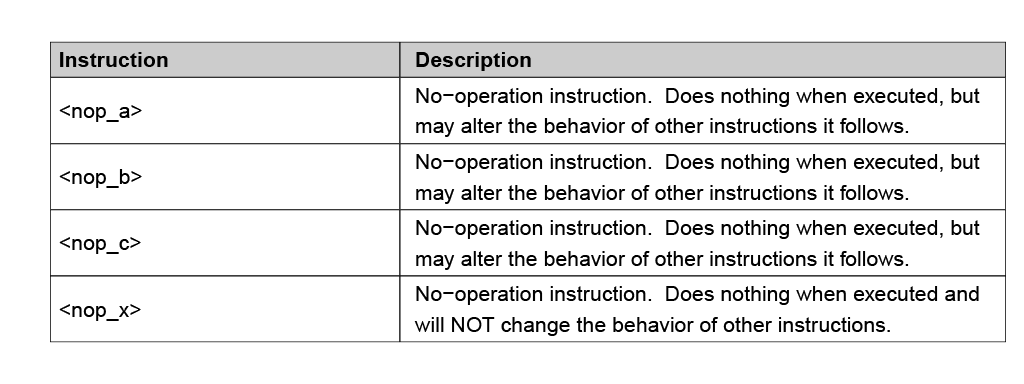
\includegraphics{images/Avida_instructions_No-operation_Table.png}
\caption{\label{fig:Avida-instructions-No-operation-Table}\textbf{No-operation instructions.} Instructions used in this study that have no direct effects when executed.}
\end{figure}

\begin{figure}
\centering
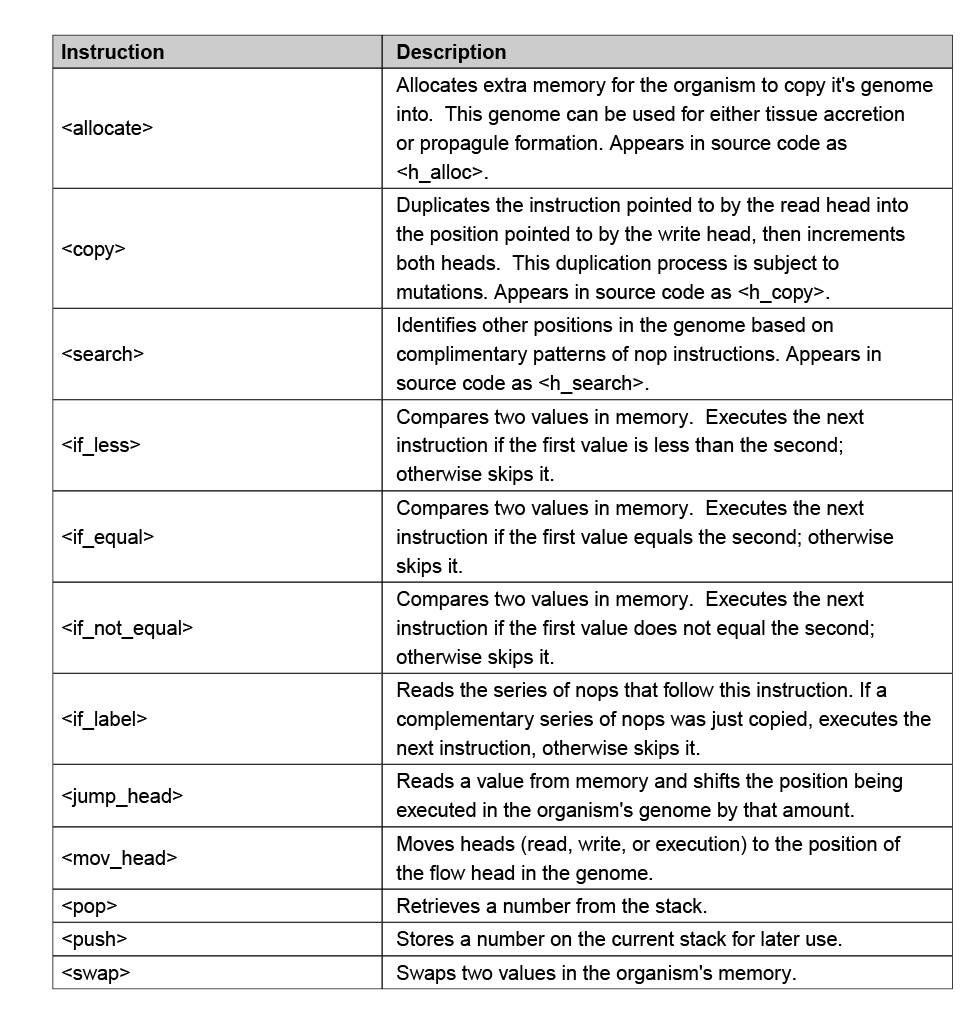
\includegraphics{images/Avida_instructions_Hardware_control_Table.png}
\caption{\label{fig:Avida-instructions-Hardware-control-Table}\textbf{Hardware control instructions.} Instructions used in this study that control the reading/writing of the Avidian genome and handle memory.}
\end{figure}

\begin{figure}
\centering
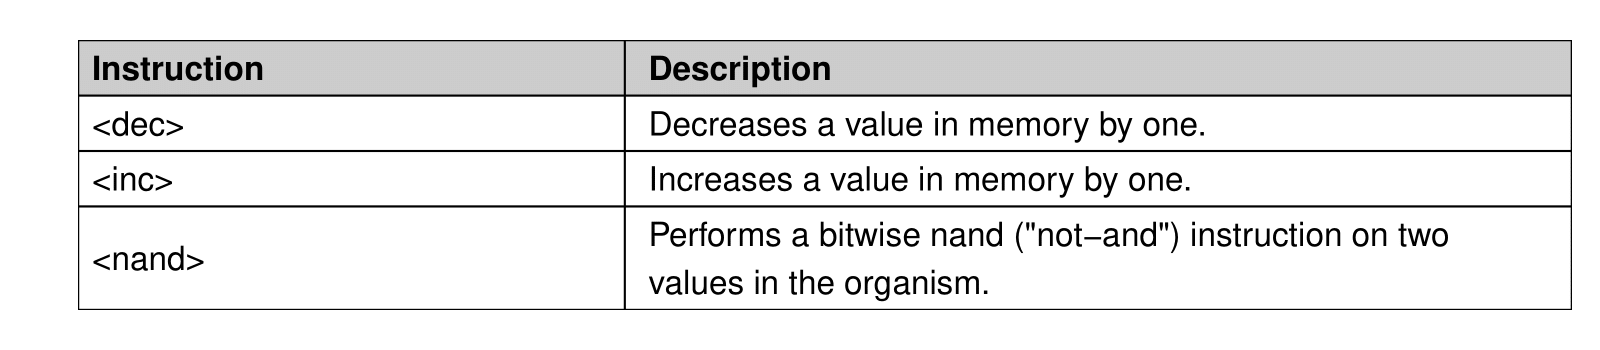
\includegraphics{images/Avida_instructions_Math_Table.png}
\caption{\label{fig:Avida-instructions-Math-Table}\textbf{Math instructions.} Instructions used in this study that execute mathematical operations.}
\end{figure}

\begin{figure}
\centering
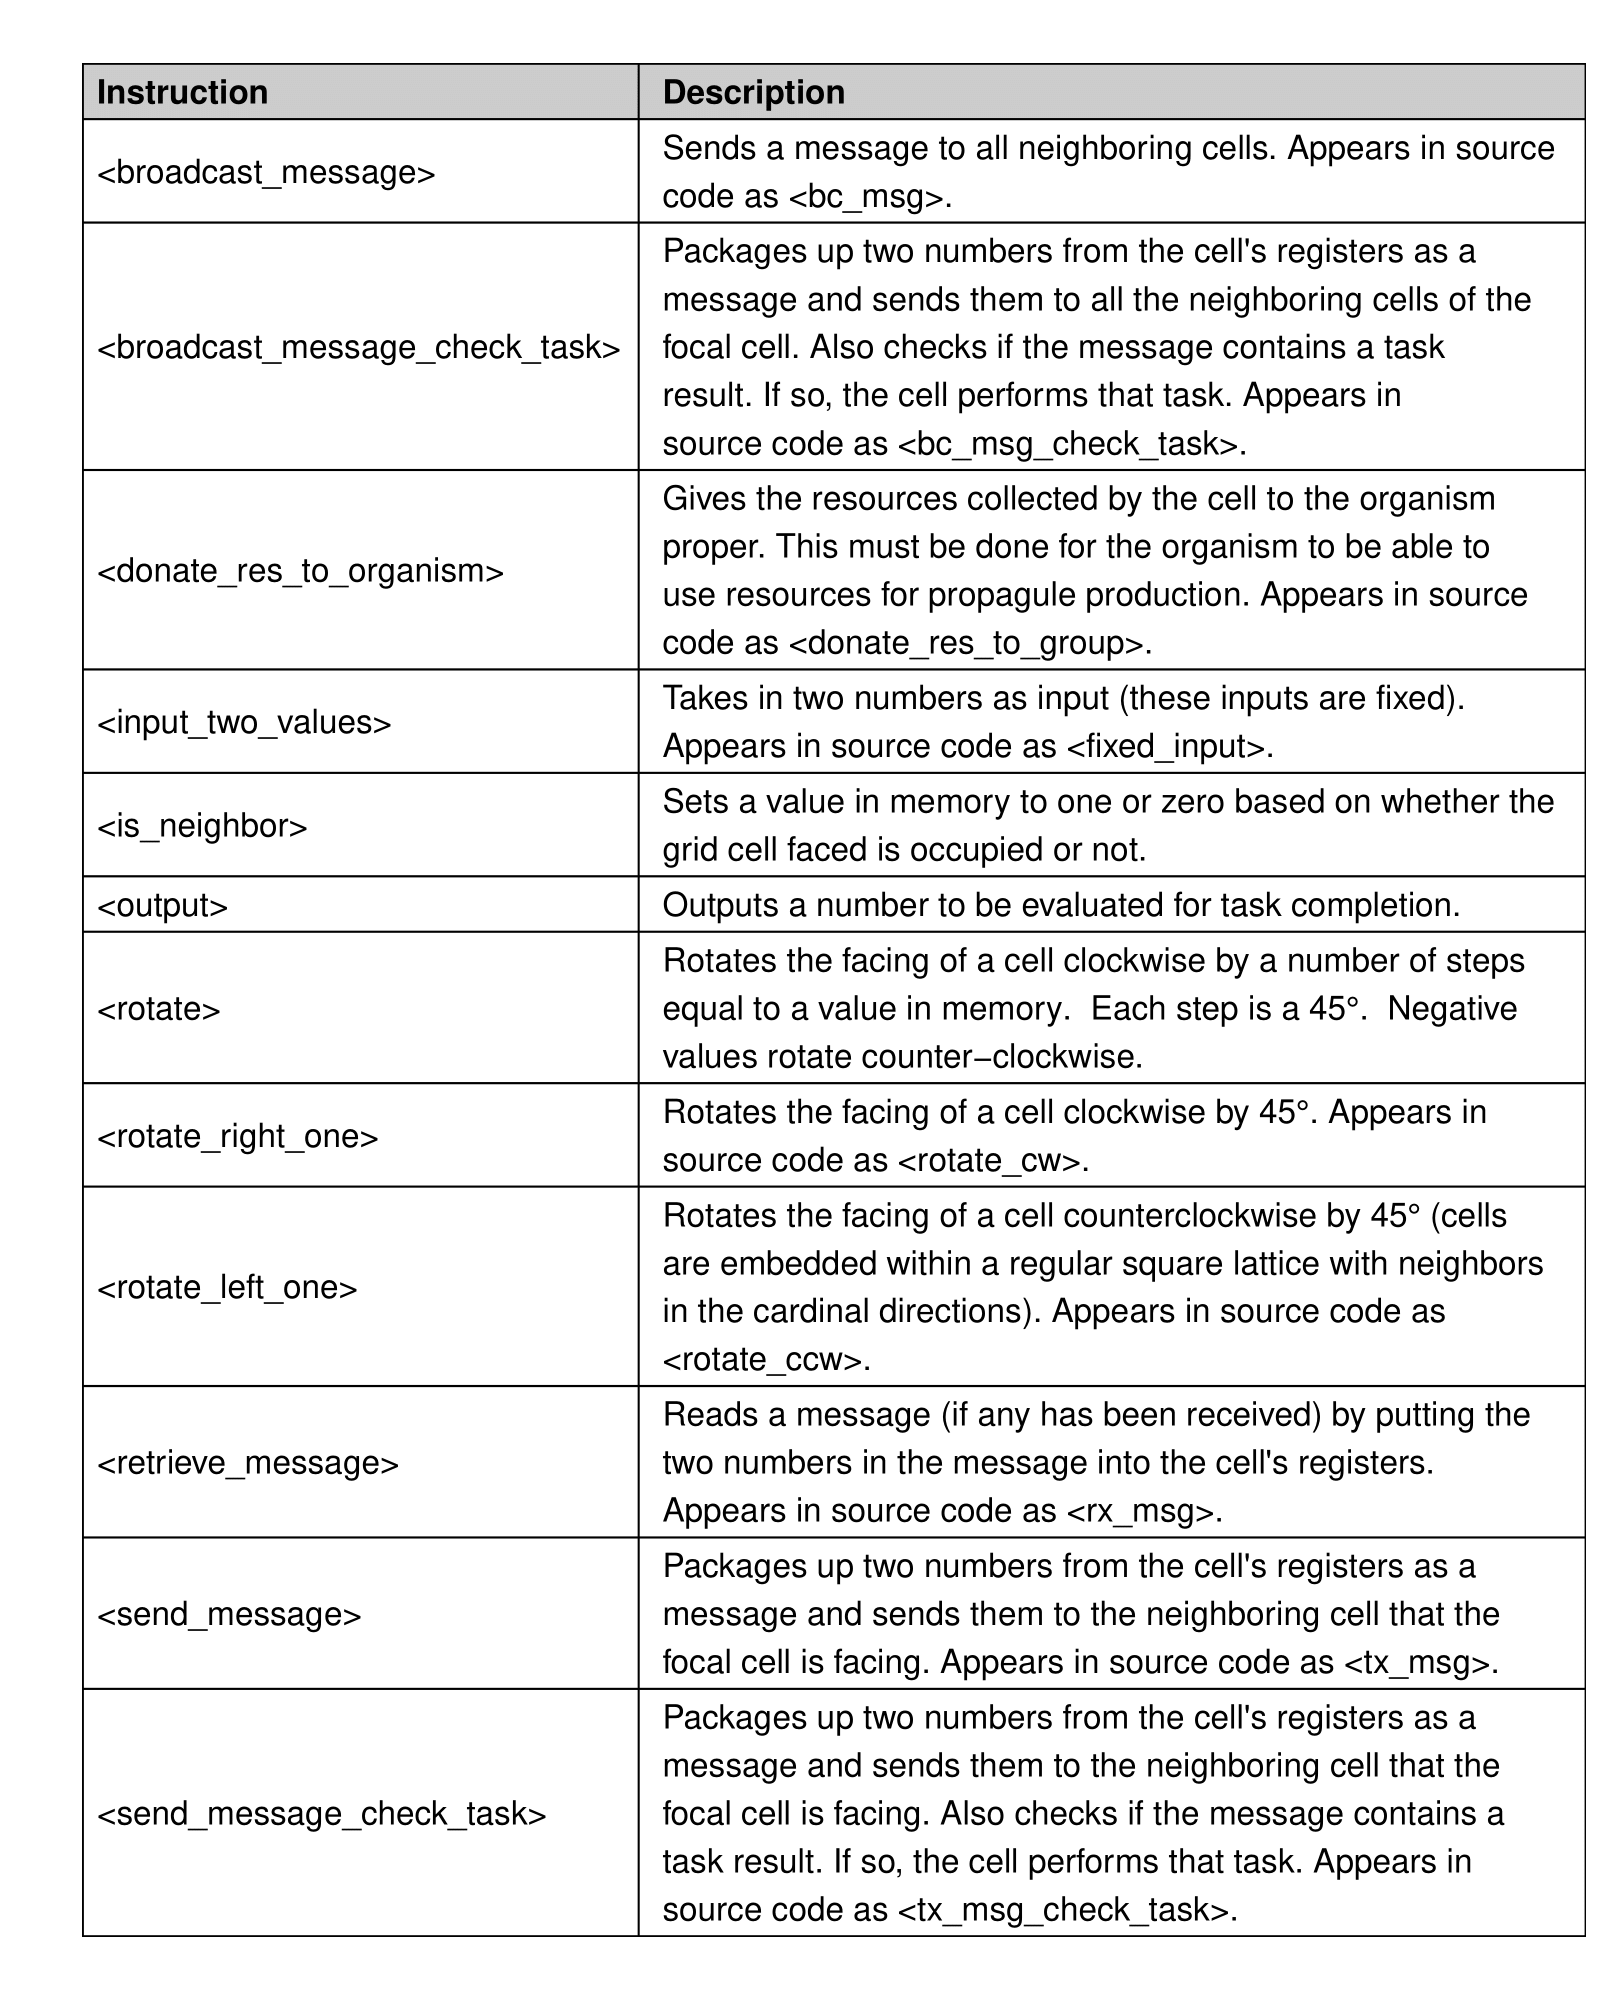
\includegraphics{images/Avida_instructions_Interaction_Table.png}
\caption{\label{fig:Avida-instructions-Interaction-Table}\textbf{Interaction instructions.} Instructions used in this study that enable communication and interaction among cells within a multicellular organism.}
\end{figure}

\begin{figure}
\centering
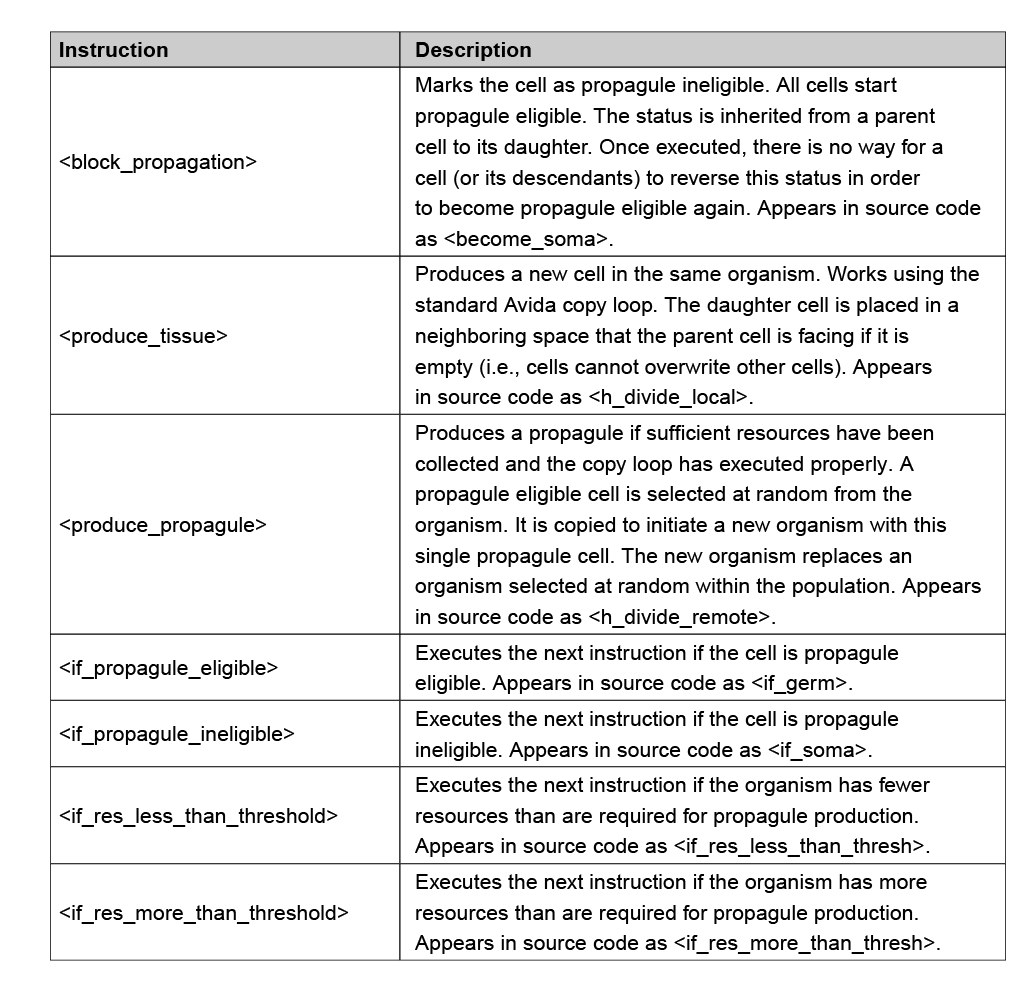
\includegraphics{images/Avida_instructions_Biological_Table.png}
\caption{\label{fig:Avida-instructions-Biological-Table}\textbf{Biological instructions.} Instructions used in this study that underpin cellular differentiation, multicellular development, and reproduction.}
\end{figure}

The metabolism of digital cells involves the completion of logic functions, where the execution of a series of genomic instructions enables the cell to export the result of a logic operation on input bitstrings. The nine possible logic functions that can be performed are NOT, NAND, AND, ORNOT, OR, ANDNOT, NOR, XOR, and EQUALS. The execution of each function enables the cell to sequester resources from a virtual resource pool, where there is one resource pool per organism per function. Each resource pool has a constant in-flow rate of one unit per update (the standard unit of time in Avida), while at the same time 1\% of the available resources flow out, limiting total accumulation to 100 units. When a cell exports the result of a function, it uptakes 5\% of the available resource associated with that function. For each function, we also specify a per-site probability of mutation each time a function is performed, referred to a ``function mutagen level'\,' (FML). Functions NOT and NAND are always non-mutagenic and thus have an FML of 0. For the treatments described in this work, the FML of the remaining seven functions increases with the complexity of the function (see Table \ref{fig:FML}. The resources acquired by successful execution of functions are required for an organism to reproduce.

\begin{figure}
\centering
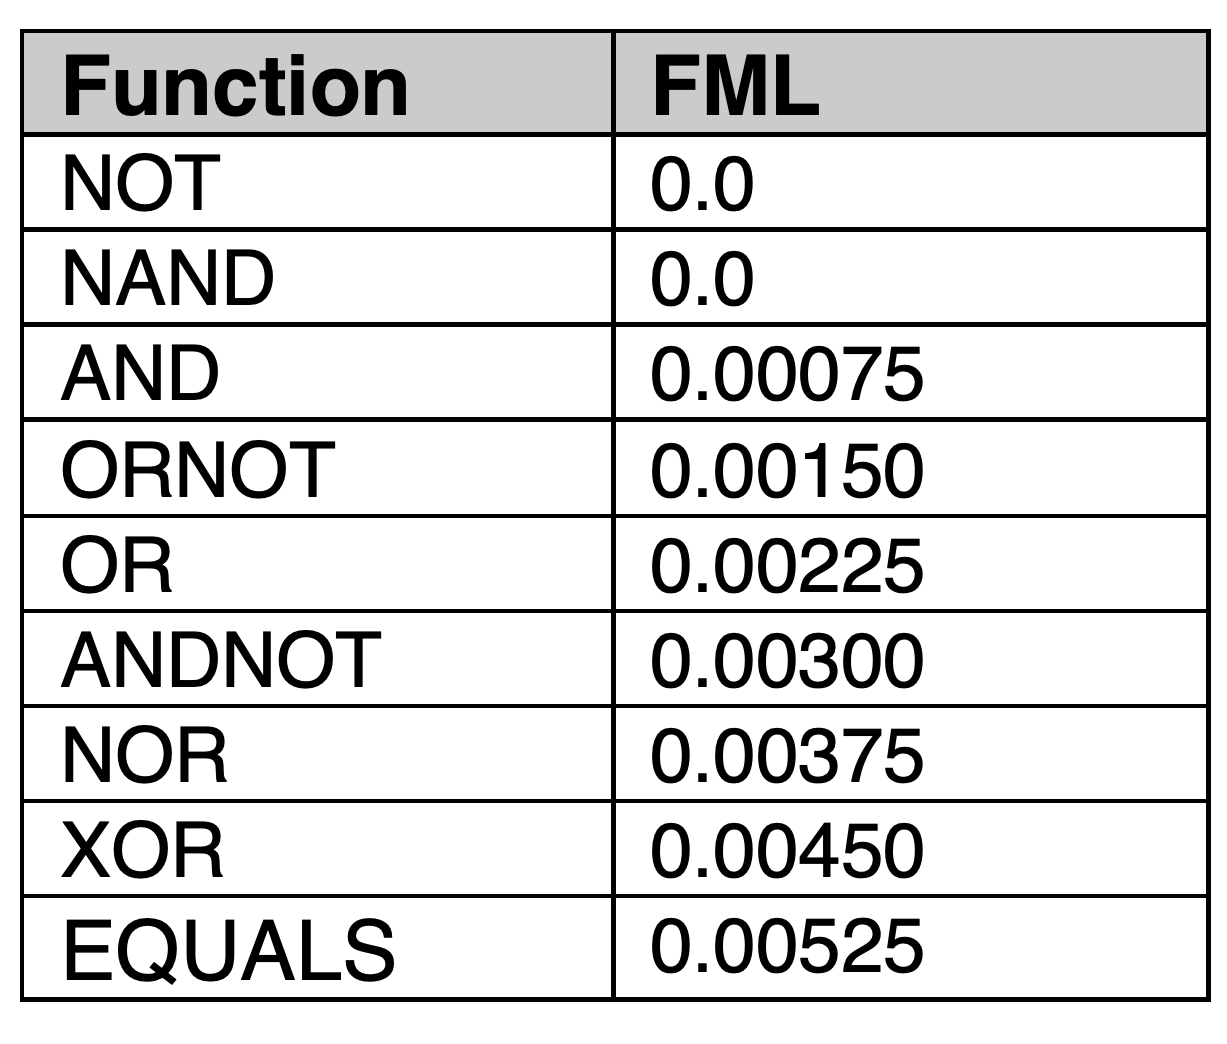
\includegraphics{images/SI_Table_FML.png}
\caption{\label{fig:FML}\textbf{Biological instructions.} Instructions used in this study that underpin cellular differentiation, multicellular development, and reproduction.}
\end{figure}

\hypertarget{workload}{%
\subsection{Workload}\label{workload}}

A cell's workload is defined as:
\[ w = \sum_{i \in F} N_i \frac{FML_i}{FML_{AND}} \]
where \(F \equiv\) \{NOT, NAND, AND, ORNOT, OR, ANDNOT, NOR, XOR, EQUALS\}, \(N_i\) is the number of times function \(i\) is performed, \(FML_i\) is the mutagenic level of function \(i\) (as specified in Table \ref{fig:FML}, and \(FML_{AND}\) is the base \(FML\) (i.e., the mutagenic level of the function AND).
We define propagule workload difference as the mean workload of propagule-ineligible cells minus the mean workload of propagule-eligible cells.

\hypertarget{mutations}{%
\subsection{Mutations}\label{mutations}}

Mutations to the genome, in which one instruction is replaced by another randomly selected instruction, occur during two different processes: organismal reproduction and the execution of ``dirty work'\,' (logic tasks with FML \(>\) 0).
Mutations during reproduction only occur during propagule production (not tissue accretion) with probability 0.01 per site. On average this results in one new mutation per propagule produced. Dirty work mutations occur immediately after a cell performs a task associated with a strictly positive function mutagen level. Each site in the genome of the performing cell experiences mutations with probability given by the FML of the task executed (Table \ref{fig:FML}. More details behind the dirty work framework are provided in Goldsby et al.~2014 \citep{goldsby2014evolutionary}.

\hypertarget{baseline-evolution-experiment}{%
\subsection{Baseline evolution experiment}\label{baseline-evolution-experiment}}

The ancestral organism is unicellular with a genome of 100 instructions. Execution of the ancestral genome initially enables only a few simple behaviors. Specifically, the ancestor completes the task NOT a single time, subsequently rotates counterclockwise and then tries to produce a propagule cell. This reproductive process fails since it only has collected \textasciitilde5 units of resource. It repeats this execution loop until it has enough resources to produce a propagule (taking roughly 1800 updates for the first generation). The population has a maximum size of 1000 organisms and evolves for a total of 1 million updates with a reproductive mutation probability of 0.01 and a dirty work mutation probability defined by whatever mutagenic functions evolve in the organisms.

\hypertarget{evolution-of-multicellularity}{%
\section{Evolution of multicellularity}\label{evolution-of-multicellularity}}

Within our system, multicellularity is generally beneficial to organisms as a result of the increased ability of multiple cells to rapidly access resources that can be devoted to propagule production. Here we explore how the efficiency of resource consumption affects the evolution of multicellularity. Within our original experiments, each cell was able to consume 5\% of the available resources each time a task was performed regardless of the number of cells in the organism. Here, we observe what happens when we increase the efficiency of resource uptake from 5\% to 8\%. This efficiency is applied at the cell level and thus is available to cells within either a unicellular or multicellular context. As can be seen in Figure \ref{fig:mc2}, increasing efficiency increases the percentage of replicates that evolve to be multicellular.

\begin{figure}
\centering
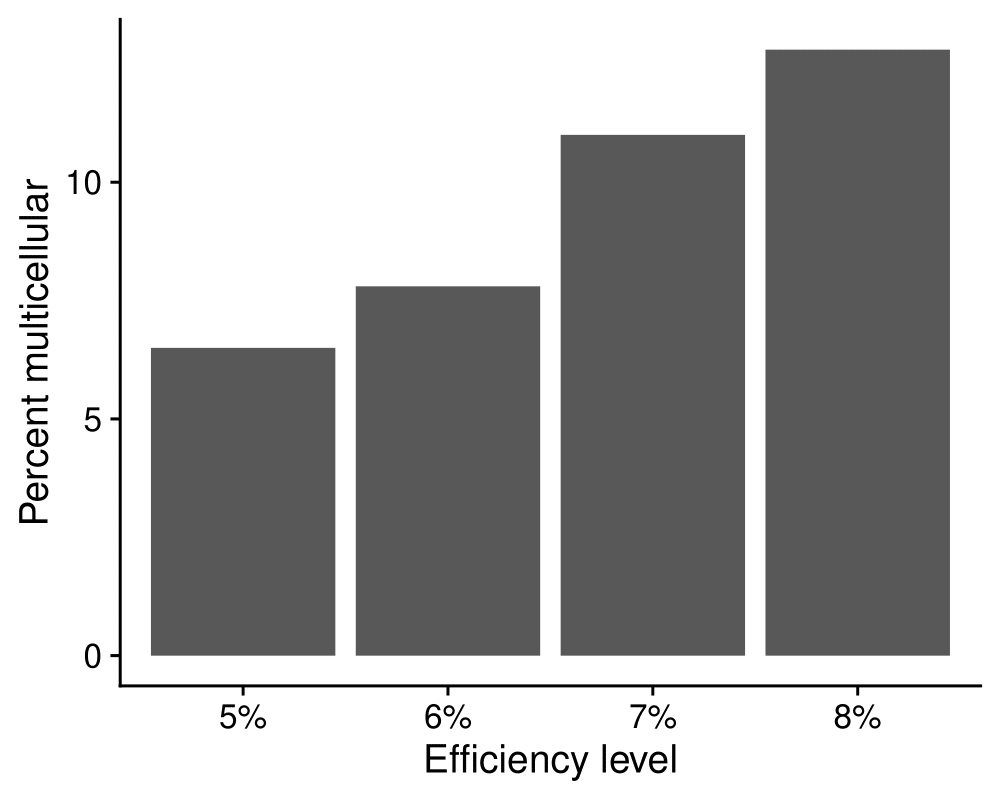
\includegraphics{images/Figure_S1_Percent_multicellular_by_efficiency_level.png}
\caption{\label{fig:mc2}\textbf{Percent of evolutionary runs that evolve multicellularity as a function of resource acquisition efficiency.} For each treatment, depicted along the x-axis, we change the efficiency with which cells are able to acquire resources, and thus the benefits of multicellularity. Our original treatment (5\%) has 1,000 replicates. The other treatments have 500 replicates. As the efficiency of resource consumption increases, so does the percentage of runs that evolve to be multicellular.}
\end{figure}

\hypertarget{cost-of-multicellularity}{%
\section{Cost of multicellularity}\label{cost-of-multicellularity}}

We added an extrinsic cost of multicellularity for the purposes of testing how readily populations would revert to back to unicells. This cost was implemented as a time delay for producing a propagule from a multicellular organism. During this delay the organism and all its constituent cells are inert -- they cannot perform tasks, acquire resources, reproduce, or communicate. Additionally, the organism remains at risk for being replaced by a reproducing competitor.

To confirm the costly nature of this time delay, we reran the evolution of our initially unicellular digital populations varying this delay from 0 updates (as in our original treatment) to 512 updates. We varied this multicellularity cost from 0 updates (as in our original evolution treatment) to 512 updates, incrementing by powers of 2 (e.g., 0, 1, 2, 4, 8, 16, etc.). As expected, fewer replicates evolved multicells as this cost was increased (Fig. \ref{fig:multi-cost}).

\begin{figure}
\centering
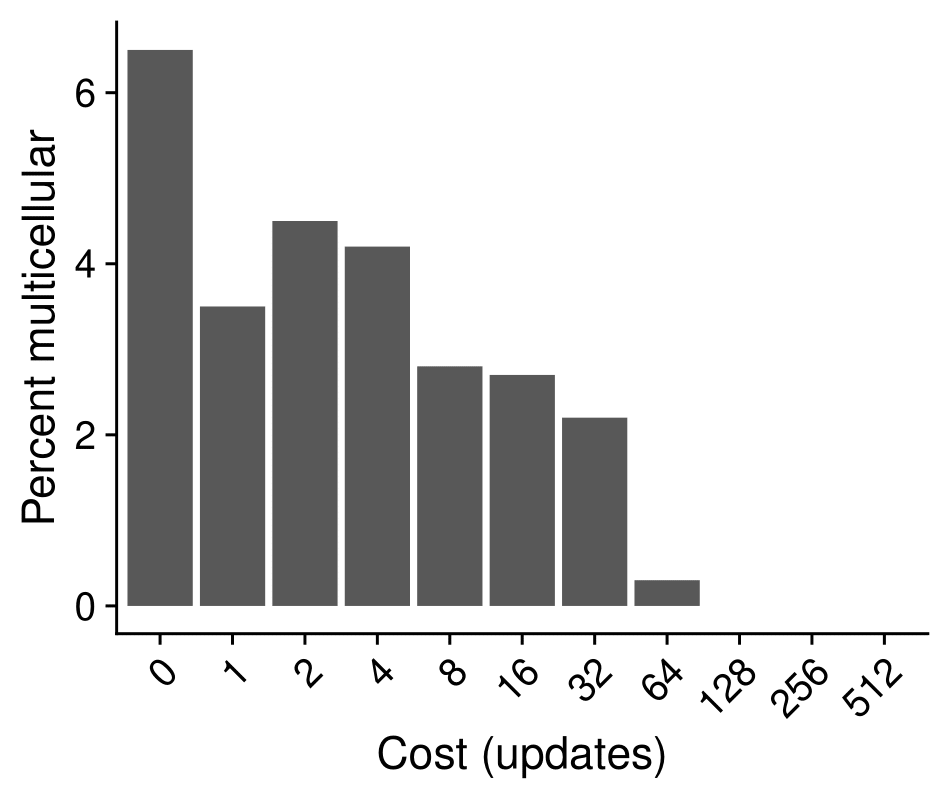
\includegraphics{images/Percent_multi_by_cost.png}
\caption{\label{fig:multi-cost}\textbf{Percent of evolutionary runs that evolve multicellularity as a function of time delay cost.} For each treatment, depicted along the x-axis, we change the cost of propagule production, and thus the benefits of multicellularity. We ran 1000 replicates of each treatment. The percentage of runs that evolve multicellularity decreases as the time delay cost increases.}
\end{figure}

\hypertarget{entrenchment}{%
\section{Entrenchment}\label{entrenchment}}

In studies of molecular evolution, a focal substitution is said to be entrenched by subsequent substitutions if it becomes relatively more deleterious to revert as a result of those subsequent substitutions \citep{shah2015contingency, flynn2017inference, starr2018pervasive, biswas2019epistasis}. Here, because we are examining the entrenchment of a \textit{phenotype} (multicellularity), we require an entrenchment metric that integrates across all possible mutations that can cause reversion to unicellularity. Specifically, we assess the degree to which multicellularity has become entrenched, by performing the following steps. First, we create a new population with 1000 copies of the organism when it was born. We then add an externally imposed cost of multicellularity. We run the population with this new multicellularity cost and observe if it reverts to unicellularity within 100 generations (assessed by measuring whether mean organism size has dropped below 2 cells after 100 generations of growth). We repeat this measurement with the following multicellularity cost values: 1, 2, 4, 8, 16, 32, 64, 128, 256, 512, 1024, 2048. To account for the stochastic nature of this assay, especially given the effect of dirty work on the organisms, we repeat the measurement three times for each organism, cost, and time point. We then compute a stability value for each genotype as the multicellular cost at which the probability of reversion to unicellularity \(= 0.5\) using a logistic fit to the data (Fig. \ref{fig:dw-entrench-comparison}). Finally, entrenchment is computed as the difference in stability value at the final and transition time points.

\begin{figure}
\centering
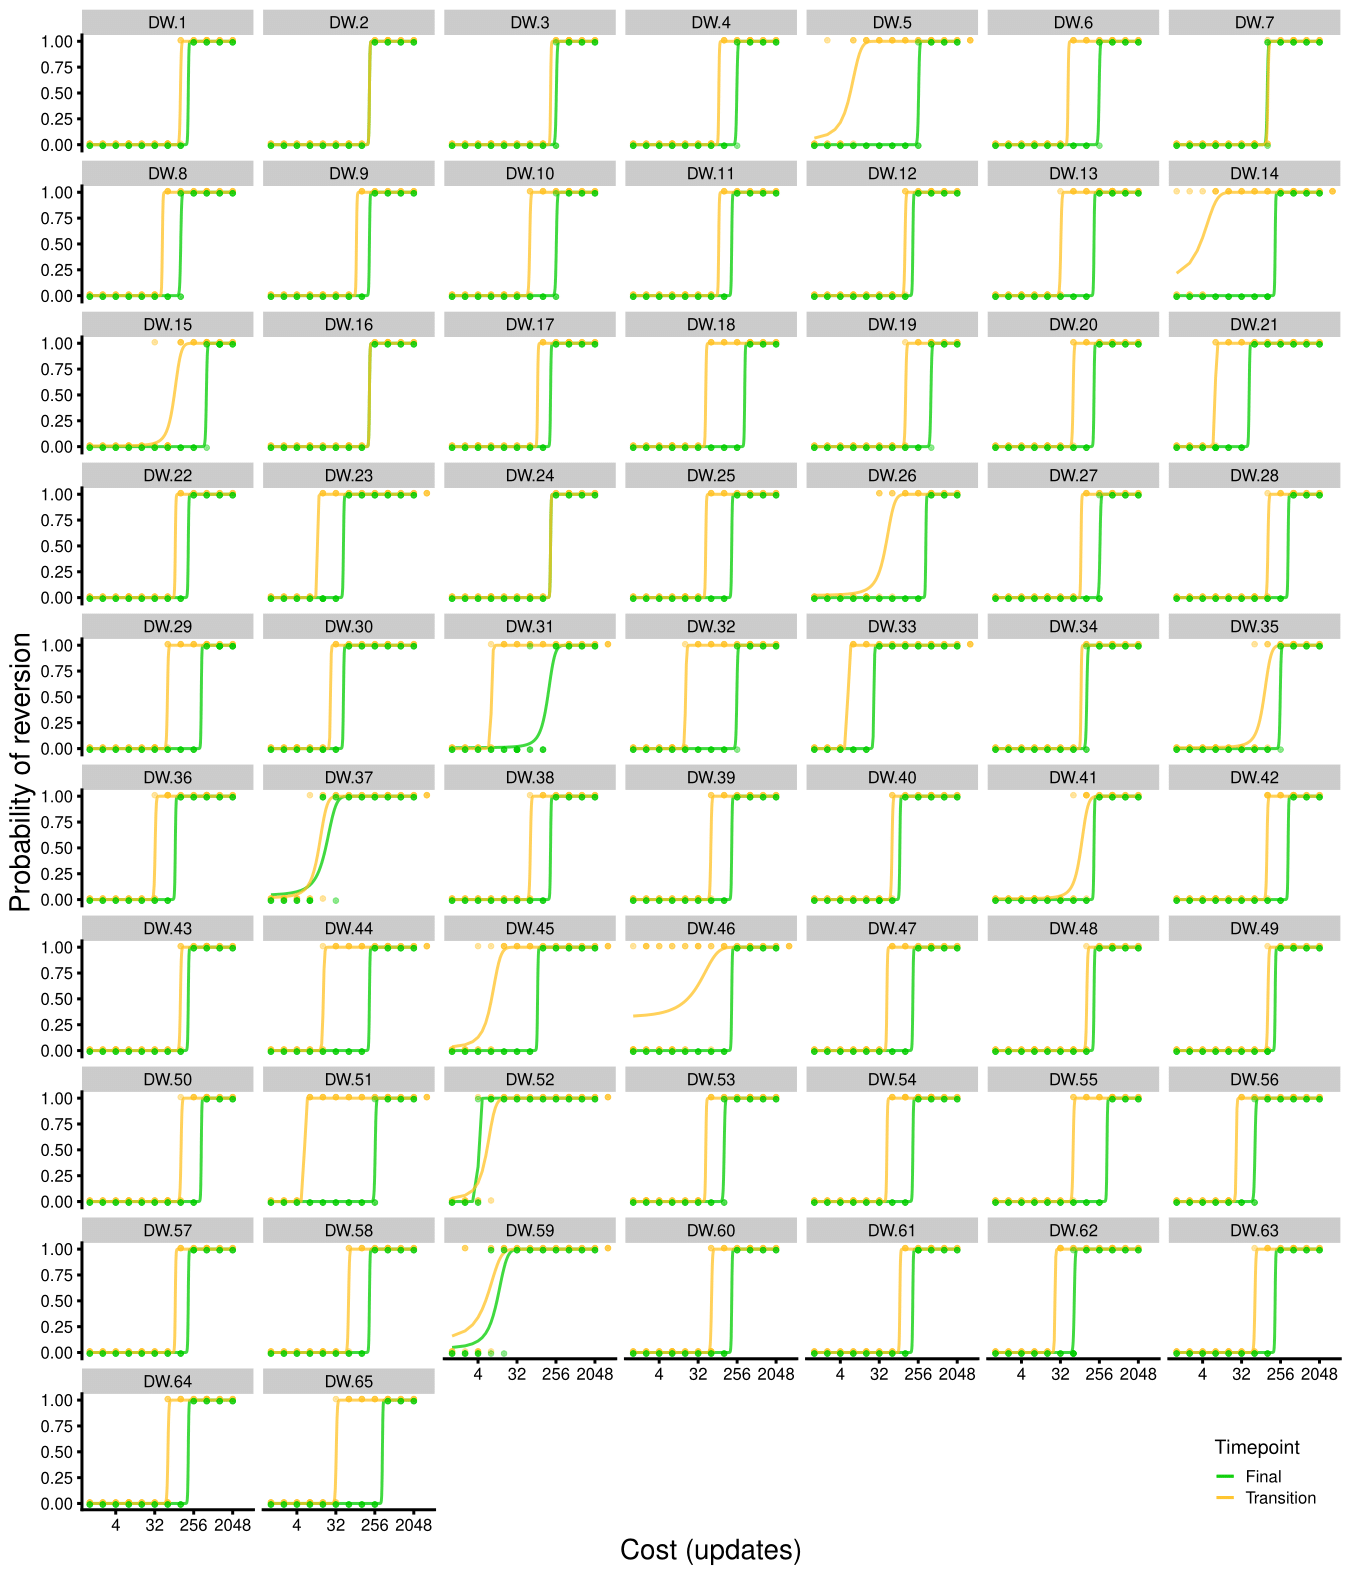
\includegraphics{images/Figure_S3_Dirty_work_Entrenchment_20DEC22.png}
\caption{\label{fig:dw-entrench-comparison}\textbf{A comparison of the stability of multicellularity at the transition and final time points of our ``Dirty Work'' evolution experiment.} The stability of multicellularity was measured for each of the 65 genotypes that evolved multicellularity at the transition (yellow) and final (green) time points of our experiment. The full range of cost values is shown with the outcomes of each replicate plotted as an indicator variable of the dominance of unicellular revertants. Logistic fits of the indicator variable are shown in yellow and green, representing the transition and final time points, respectively.}
\end{figure}

\hypertarget{generation-and-assessment-of-unicellular-revertants}{%
\section{Generation and assessment of unicellular revertants}\label{generation-and-assessment-of-unicellular-revertants}}

To understand the forces that govern whether or not a multicell is entrenched, we create all possible single-locus mutants at two time points: the ``transitional'' multicellular organism along the line of descent of the dominant multicell and ``final'' multicellular organism within this same lineage. For each single-locus mutant, we assess its viability as well as its fitness.

The first step in the assessment pipeline is the viability assay, which is a simple test to rule out organisms that are nonviable from further computationally expensive assessment. To assess a mutant's viability, we run the mutated genome for an extended period of time (up to 10,000 updates) without mutations occurring as the result of dirty work. If, within this time period, the mutated organism is able to accumulate the resources required for reproduction and to execute the instruction to create a new organism, we consider it viable and stop the viability assay. Viable mutants are then further classified as either multicellular (indicating that it executed tissue accretion instructions resulting in cellular reproduction and thus contains more than two cells) or unicellular.

This viability assay is used as a gateway to further screening and thus its conclusions are refined by the subsequent growth assay. For example, since the organism is running its code in isolation it does not actually produce an offspring organism. Additionally, it may not contain propagule-eligible cells and thus may not be able to produce offspring when grown in a population under standard conditions. If so, later assays will classify it as nonviable. Similarly, the organism may be unicellular at the time of its first successful execution of the propagule production instruction and may later execute tissue accretion instructions, becoming multicellular. If so, later assays will classify it as multicellular.

\hypertarget{growth-assay-and-measuring-relative-fitness}{%
\subsection{Growth assay and measuring relative fitness}\label{growth-assay-and-measuring-relative-fitness}}

To measure the fitness of a multicellular progenitor strain or a unicellular revertant strain, we create a solitary organism with the genome of interest and place it into an empty population with room for 62 organisms. The organism is allowed up to 50,000 updates to reach a population size threshold of 32 organisms. Once this threshold is reached, or exceeded (multiple simultaneous reproduction events can push populations above the 32 organism threshold), we calculate the average rate of increase, or Malthusian parameter, \(M\), as
\begin{equation}
\ M = log(N_f / N_i )/T
\end{equation}
where \(N_f\) and \(N_i\) are the final and initial number of organisms in the population and \(T\) is the time it took the organism to fill the entire population. In the case that the organism fails to fill the entire population by the end of the growth assay, \(T\) is set to the maximum allowed time of 50,000 updates.

To account for the effects of mutation, we repeat this process 100 times for each unicell revertant genotype and its multicell progenitor strain with different random number ``seeds,'\,' leading to a different set of mutations and different cell behaviors. The fitness of a given unicell revertant relative to its multicell progenitor is defined as the ratio of their average Malthusian parameters across these replicate measurements.

\hypertarget{identification-of-unicellular-revertants}{%
\subsection{Identification of unicellular revertants}\label{identification-of-unicellular-revertants}}

Some mutations that occur over the course of the growth assay could result in data that may no longer be suitable for our analyses. For example, mutations that cause an organism to re-evolve multicellularity can occur during the growth assay, confounding our ability to accurately measure the relative fitness of \textit{unicellular} revertants. Another potentially confounding scenario is that the organism we initiate the population with may fail to divide in the allotted time. This can occur if the initial organism flags itself as ``propagule ineligible'' or if it incurs a lethal mutation, as a result of dirty work, prior to the first propagule production event. To avoid these potentially confounding effects, we employ a two-step data filtering pipeline.

We begin by assessing whether the organisms in the population have remained unicellular for the entire duration of the growth assay. To do this, we check that the total number of cells in the population at the end of the growth assay is not greater than the total number of organisms. In total, \textasciitilde42.5\% of our growth rate assays are ``contaminated'' with re-evolved multicells. We see considerable diversity within our unicell revertant genotypes; a single unicell genotype can produce a variety of outcomes: some which remain unicellular and others which re-evolve multicellularity. This is fully in line with our expectation that different mutations will occur in organisms started with different random seeds. While some multicellular progenitor genotypes appear to produce revertants that re-evolve multicellularity at higher rates than others, we find that the probability distributions for re-evolving multicellularity are quite similar at the transition and final time points (Fig. \ref{fig:dw-filter-1-reevolving-multicellularity}).

\begin{figure}
\centering
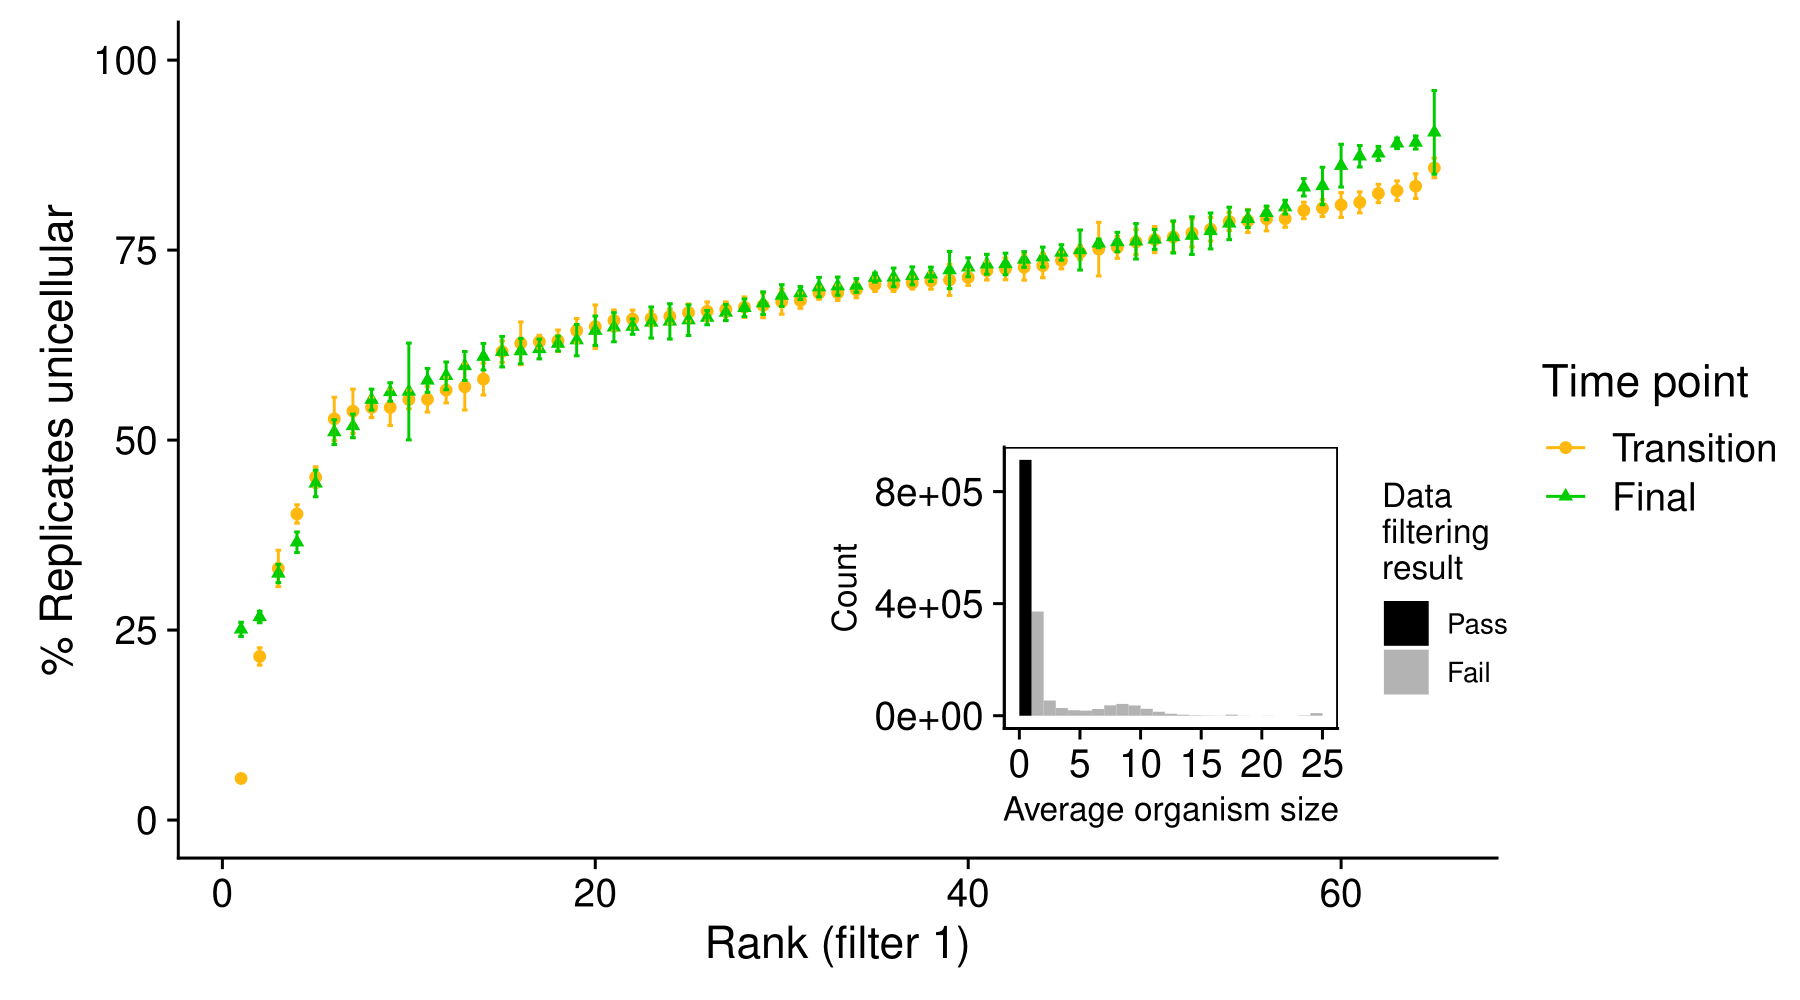
\includegraphics{images/Figure_S4_Dirty_work_Populations_that_re-evolve_multicellularity_NEW_14MAR23.png}
\caption{\label{fig:dw-filter-1-reevolving-multicellularity}\textbf{Filtering unicellular revertants from the ``Dirty Work'' experiment that re-evolve multicellularity.} The mean and standard error for the percent of replicate populations that remain unicellular for the transition (yellow) and final (green) time points of our experiment. Unicellular revertant genotypes are grouped according to their multicellular parental genotypes and ranked from least to most replicates that remain unicellluar for each time point independently. \textbf{Inset} Schematic representation of our filtering criterion using data aggregated across all genotypes and both time points. We filter out any population in which the average organism size exceeds 1, indicating that multicellularity has re-evolved. Grey color indicates replicates that fail to pass the filter, black indicates those that do.}
\end{figure}

We next determine whether the organisms used to initiate the population have successfully reproduced at least once in the allotted 50,000 generations. To do this, we simply check that the total number of cells in the population is greater than 1. In total, 19\% of our remaining replicate populations fail to successfully reproduce. As above, we find that some multicell progenitor genotypes are more likely than others to produce unicellular revertants that fail to successfully reproduce. However, in this case, we find that multicells from the final time point are more likely to produce inviable unicellular revertants than transition multicells (Fig. \ref{fig:dw-filter-2-failure-to-divide}).

\begin{figure}
\centering
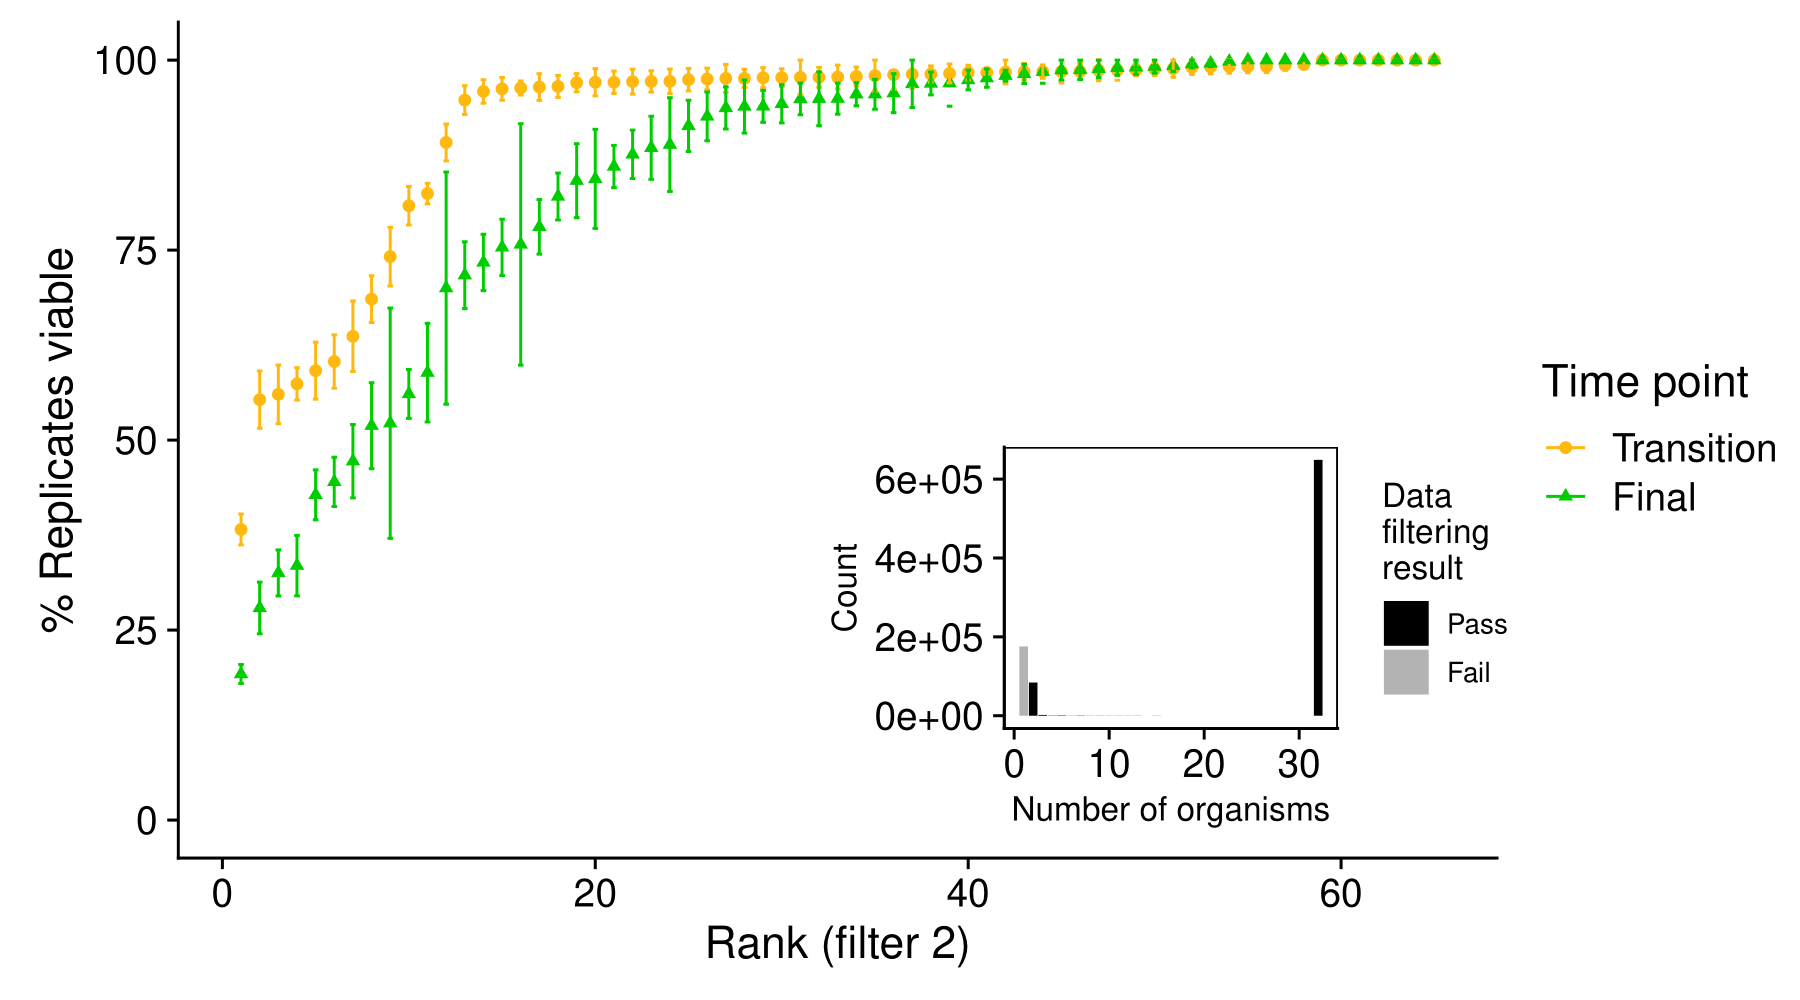
\includegraphics{images/Figure_S5_Dirty_work_Populations_that_fail_to_divide_NEW_14MAR23.png}
\caption{\label{fig:dw-filter-2-failure-to-divide}\textbf{Filtering unicellular revertants from the ``Dirty Work'' experiment that fail to reproduce.} The mean and standard error for the percent of replicate populations that successfully reproduce for the transition (yellow) and final (green) time points of our experiment. Unicellular revertant genotypes are grouped according to their multicellular parental genotypes and ranked from least to most replicates that remain unicellluar for each time point independently. \textbf{Inset} Schematic representation of our filtering criterion using data aggregated across all genotypes and both time points. We filter out any population in which the number of organisms at the end of the growth assay is less than 2, indicating that the organism that seeded the population has failed to reproduce. Grey color indicates replicates that fail to pass the filter, black indicates those that do.}
\end{figure}

\hypertarget{distribution-of-fitness-effects-of-unicellular-reversion-mutations}{%
\section{Distribution of fitness effects of unicellular reversion mutations}\label{distribution-of-fitness-effects-of-unicellular-reversion-mutations}}

Using only the runs that passed both of our quality control filters (see text above), we then explored the distribution of fitness effects of reversion mutations for each multicellular lineage at the time of the transition to multicellularity and at the final time point of the evolutionary run (Fig. \ref{fig:dw-DFERMs}.

\begin{figure}
\centering
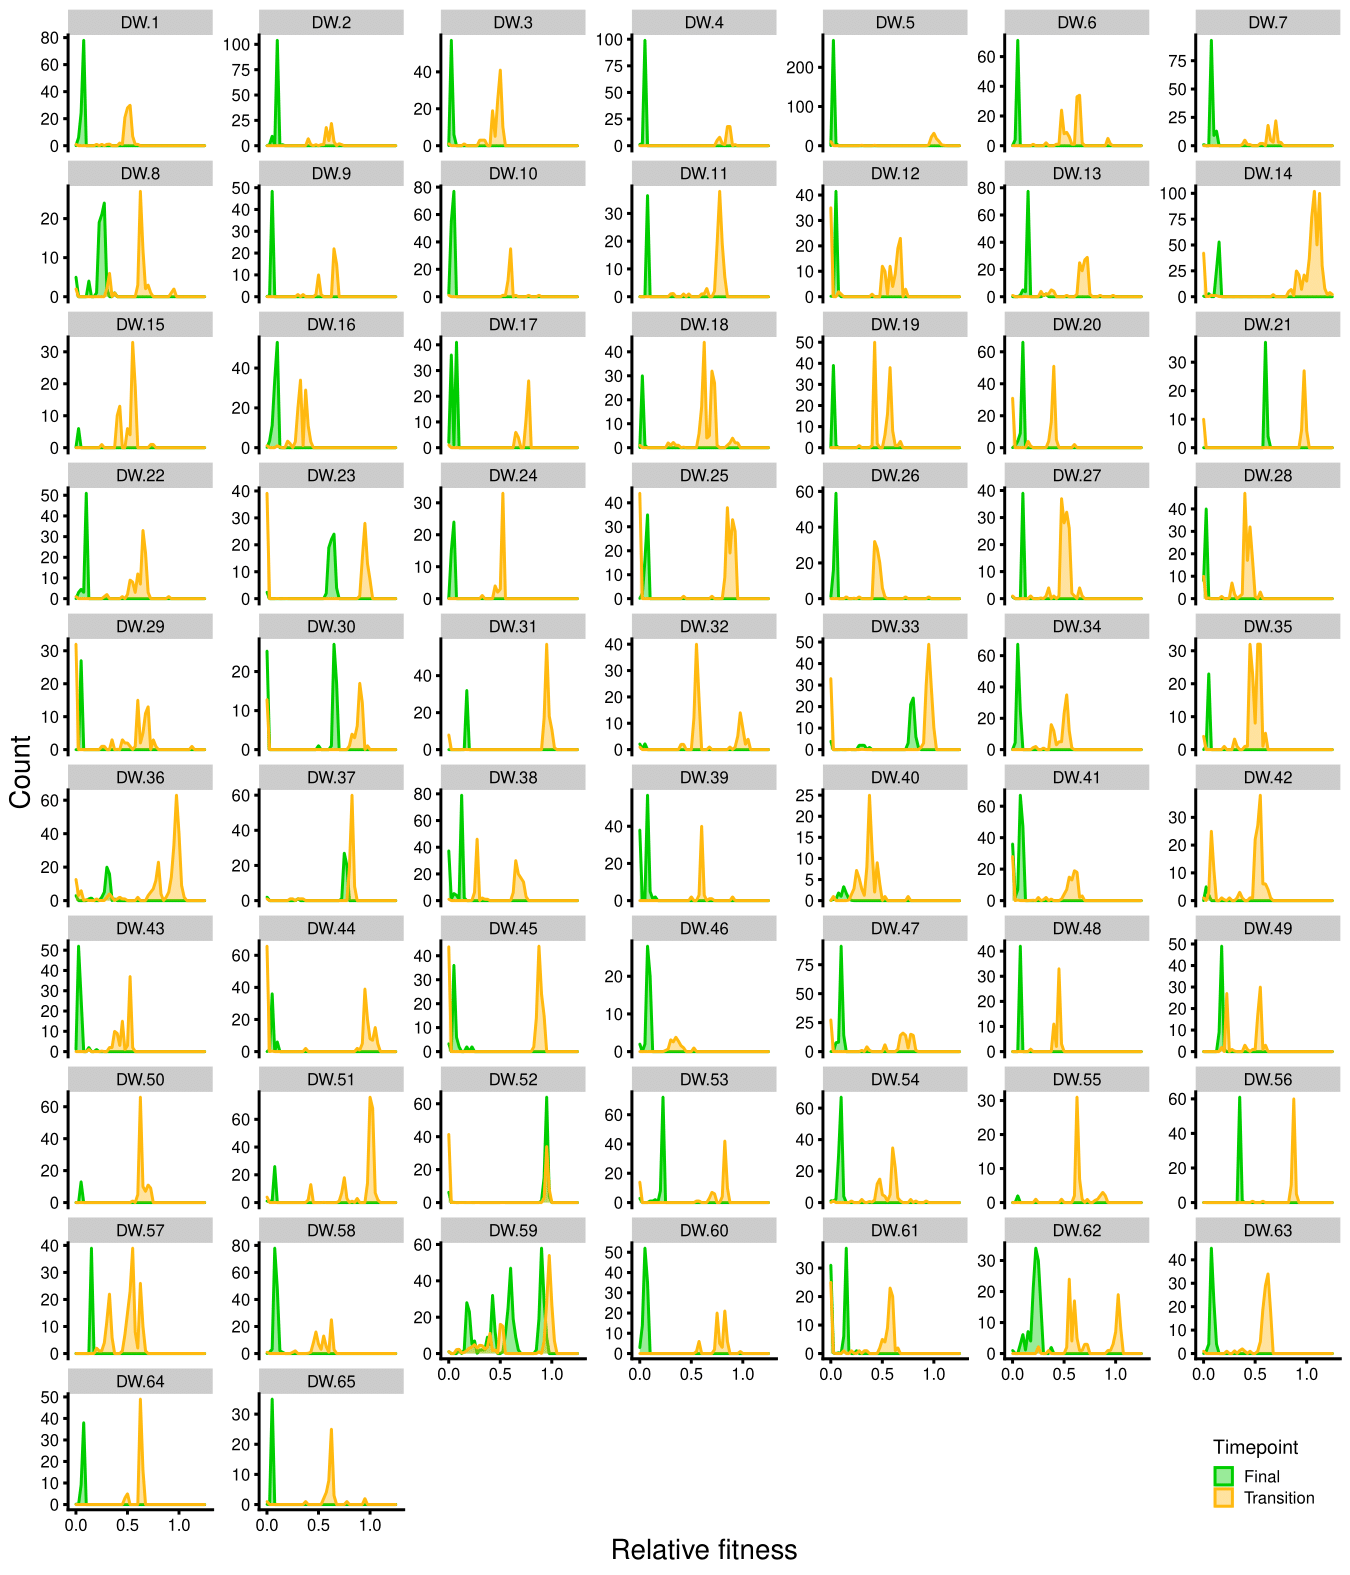
\includegraphics{images/Figure_S6_Relative_fitness_distributions_20DEC22.png}
\caption{\label{fig:dw-DFERMs}\textbf{Distribution of fitness effects of unicellular reversion mutations from the ``Dirty Work'' experiment at the transition and final time points.} The empirical distribution of fitness effects of reversion mutations for each lineage that evolved multicellularity in our ``Dirty work'' experiment. Yellow indicates the distribution at the transition point, green at the final time point. Counts are proportional to the adjusted number of unicellular revertants.}
\end{figure}

\hypertarget{reversion-mutation-identities-and-the-determinants-of-the-number-of-viable-reversion-mutations}{%
\section{Reversion mutation identities and the determinants of the number of viable reversion mutations}\label{reversion-mutation-identities-and-the-determinants-of-the-number-of-viable-reversion-mutations}}

To further understand the determinants of the number of viable reversion mutations, we explored the identity of the mutations that caused reversion from multicellularity to unicellularity at the transition and final time points of our experiment. For each time point we recorded the following: the identity of the mutant operation that caused reversion, the identity of the wild-type operation that was replaced, and the position in the genome. Figure \ref{fig:case-study-reversion-mutation-identities} gives a representative example reversion mutation network for our case study lineage at the final time point which highlights 3 major categories of mutation that lead to a reversion to unicellularity. First, the \(<h\_divide\_remote>\) operation, which encodes propagule production, can be inserted at several sites in the genome (usually upstream of the operation encoding tissue accretion) to repress tissue accretion in a dominant epistatic manner. Second, the regulatory loci controlling the expression of tissue accretion can be disrupted (e.g., the loss of the \(<if\_res\_less\_than\_thresh>\) operation at position 12 in our final case study genome). Third, loss-of-function mutations occur when the tissue accretion operation, \(<h\_divide\_local>\), is substituted for another operation that does not disrupt propagule production.

When we look at the spectrum of reversion mutations across all 65 lineages that evolved multicellularity, we find that the same basic pattern emerges at both the transition and final time points (Figs. \ref{fig:reversion-mutation-identities}-\ref{fig:wt-operation-identities}). Loss-of-function mutations are the most common cause of reversion followed closely by dominant epistatic mutations. Changes in regulatory elements make up the third most common category of reversion mutation and occur at a slightly higher frequency in the final genomes than the transition genomes. The biggest difference in mutation spectrum between the transition and final time points is in the frequency at which \(<nop\_x>\) operations are replaced (Fig. \ref{fig:wt-operation-identities}). However, this difference is caused by the fact that the ancestral unicell that was used to initiate each evolutionary run had an extremely minimal genome composed largely of \(<nop\_x>\) operations (a null operation). These large blocks of null operations are gradually replaced over time as the population evolves; thus, earlier time points will contain more null operations than later ones. When adjusted for the frequency of the \(<nop\_x>\) operation in the multicell genomes (\(24.4\%\) at the time of transition vs.~\(1.9\%\) at the final time point), the difference in frequency effectively goes to zero.

Another factor we hypothesized could lead to a decrease in the number of viable reversion mutations was the presence of redundant tissue accretion mutations. Since the primary routes to achieving unicellularity involve replacing or silencing the expression of the tissue accretion instruction, it is possible that multicells could become more robust to reversion by accumulating secondary functional copies of the \(<h\_divide\_local>\) operation. We found some evidence of a trend in this direction (Fig. \ref{fig:redundant-tissue-accretion-instructions}).

\textcolor{red}{\textbf{Note to Heather: Please help!} Four genotypes (4310T, 3038F, 4278F, and 4310F) had a total of 147 reversion mutations that did not map to any existing position in their consensus genomes. These errors make up ~1.16\% of the total number of reversion mutations in our study.}

\begin{figure}
\centering
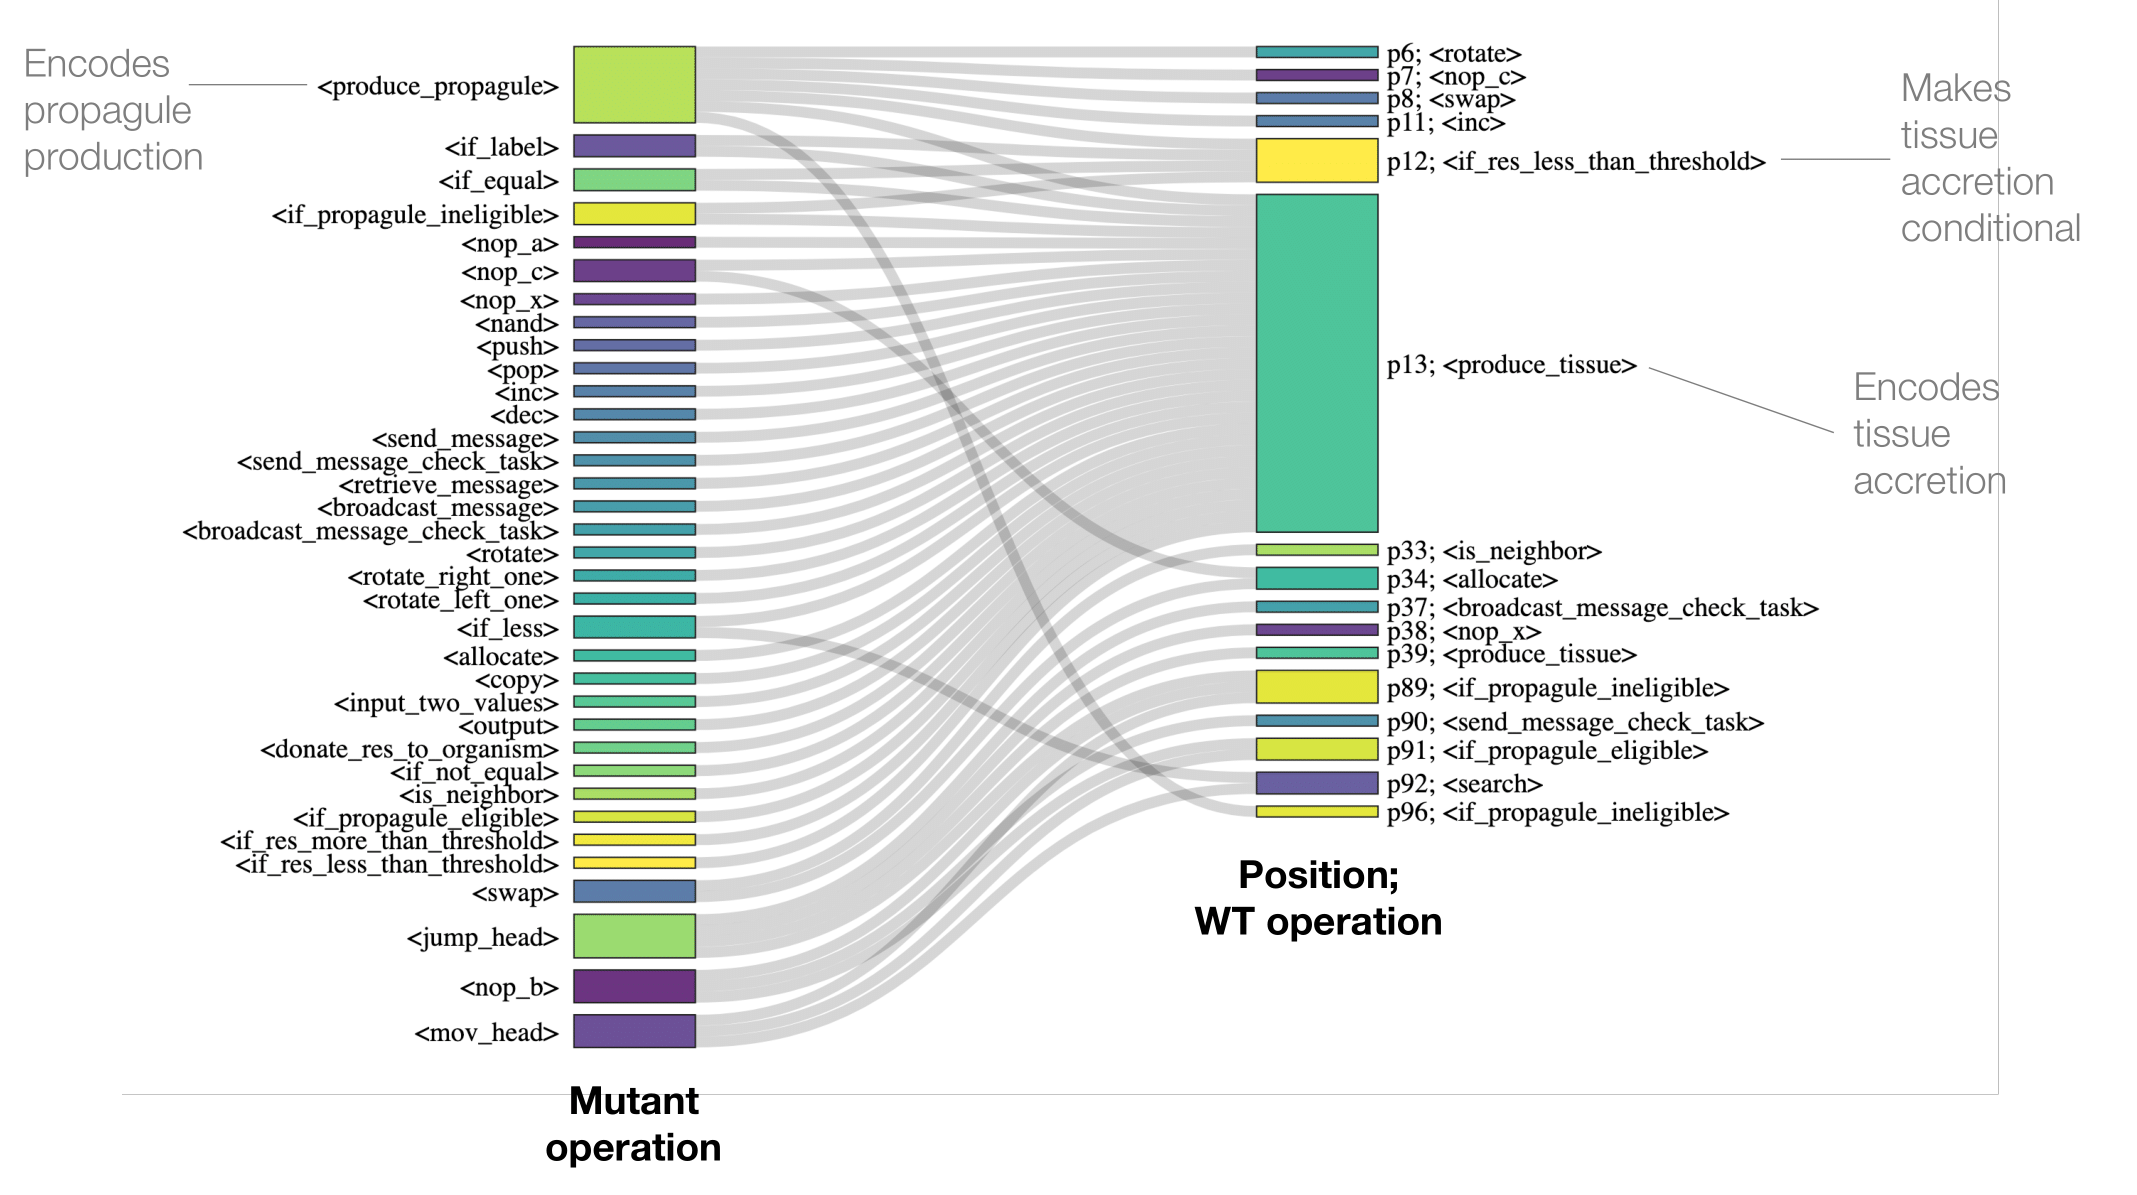
\includegraphics{images/Final_case_study_mutation_network_30DEC22.png}
\caption{\label{fig:case-study-reversion-mutation-identities}\textbf{Identities of the mutations that caused reversion to unicellularity in our case study lineage at the final time point.} Here we show how the reversion mutations map onto the positions in the genome that were mutated and the operations they replaced for our case study. The color of each node corresponds to the operation and genome position is labeled for each operation that was replaced in the final multicell genome.}
\end{figure}

\begin{figure}
\centering
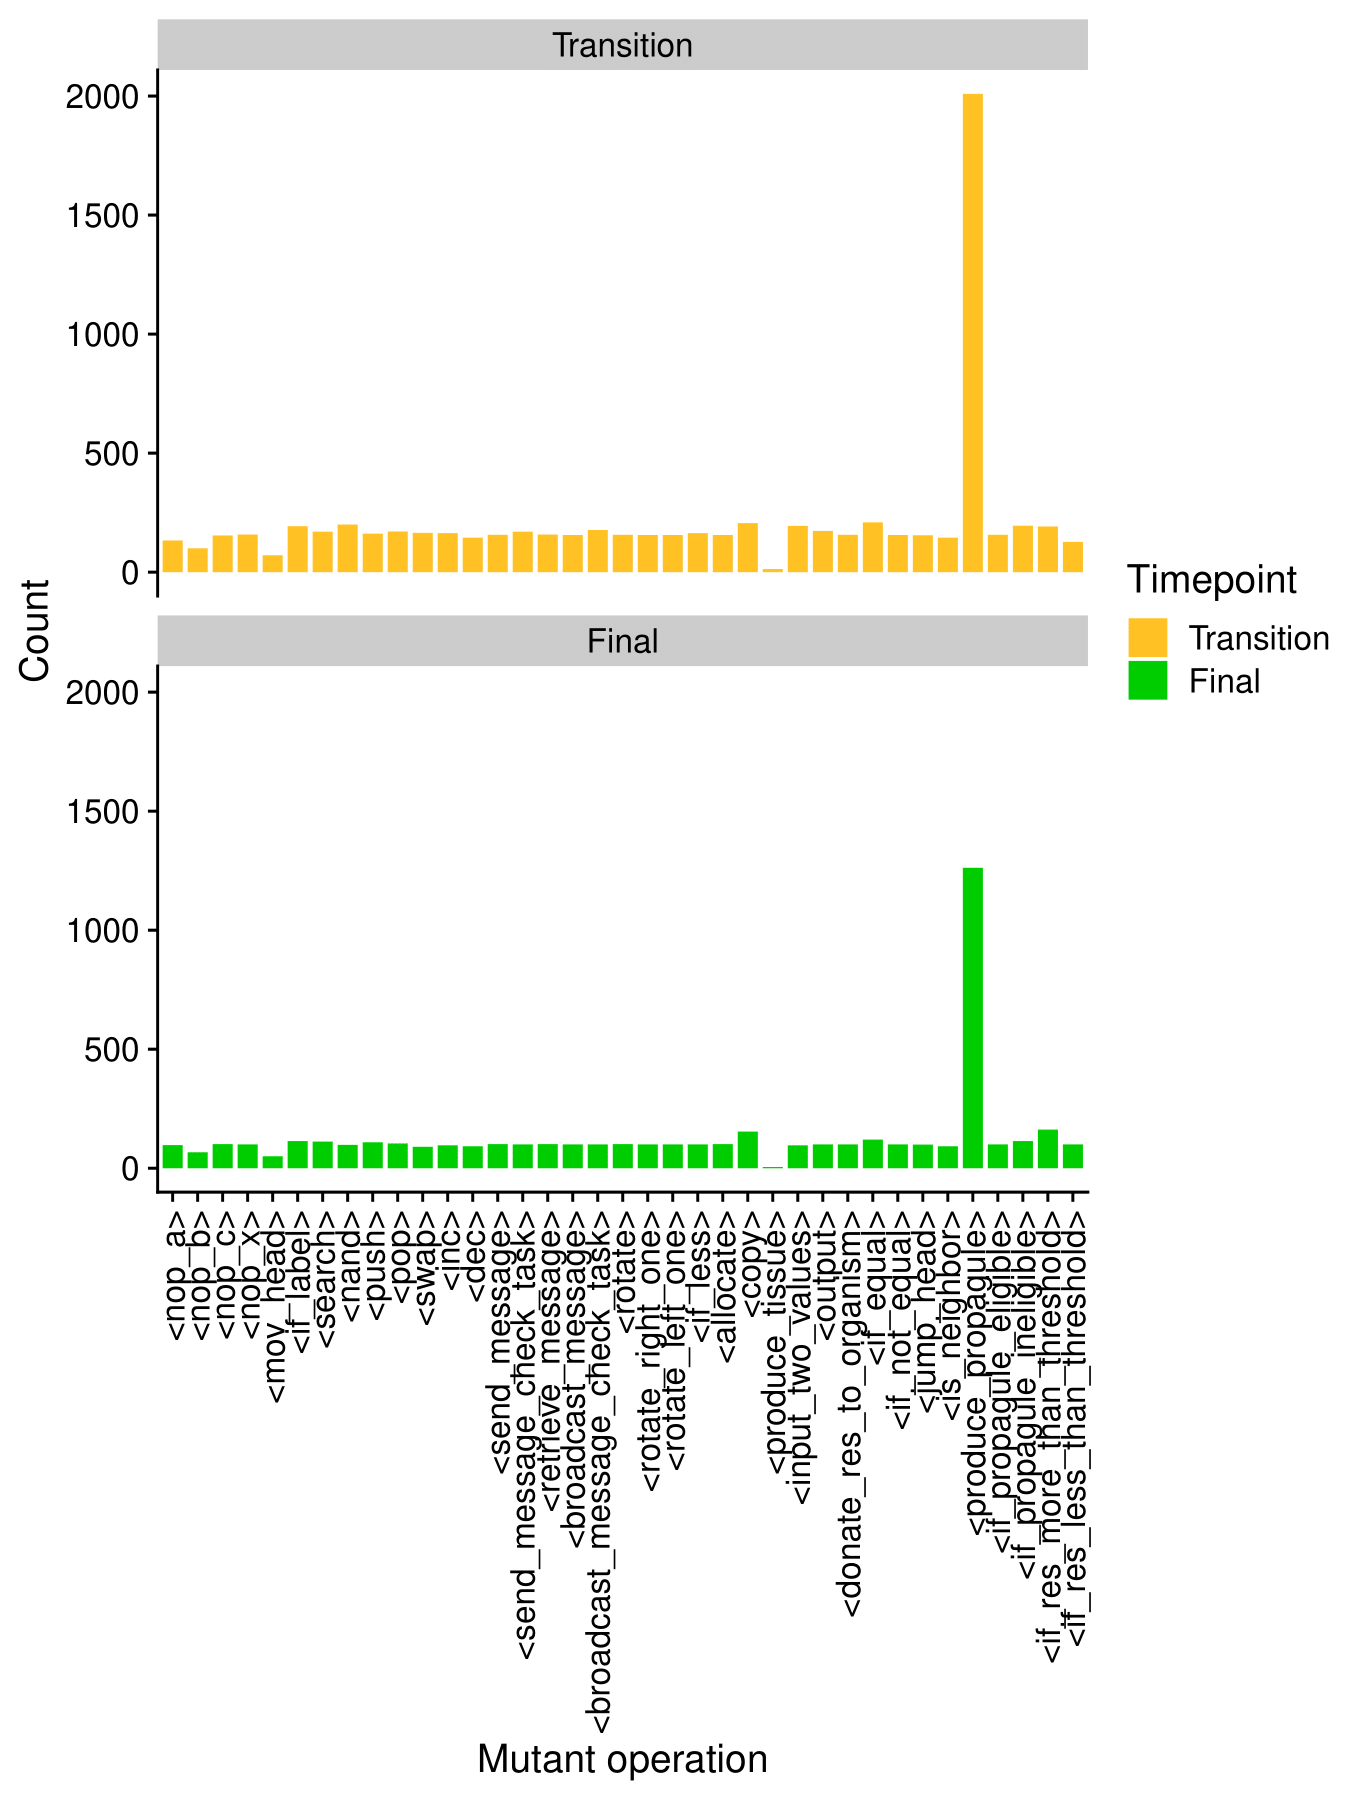
\includegraphics{images/Mutant_operations_at_transition_and_final_time_point_20DEC22.png}
\caption{\label{fig:reversion-mutation-identities}\textbf{Changes in reversion mutation identities from the transition to final time point.} The number of times different mutant operations caused reversion to unicellularity.}
\end{figure}

\begin{figure}
\centering
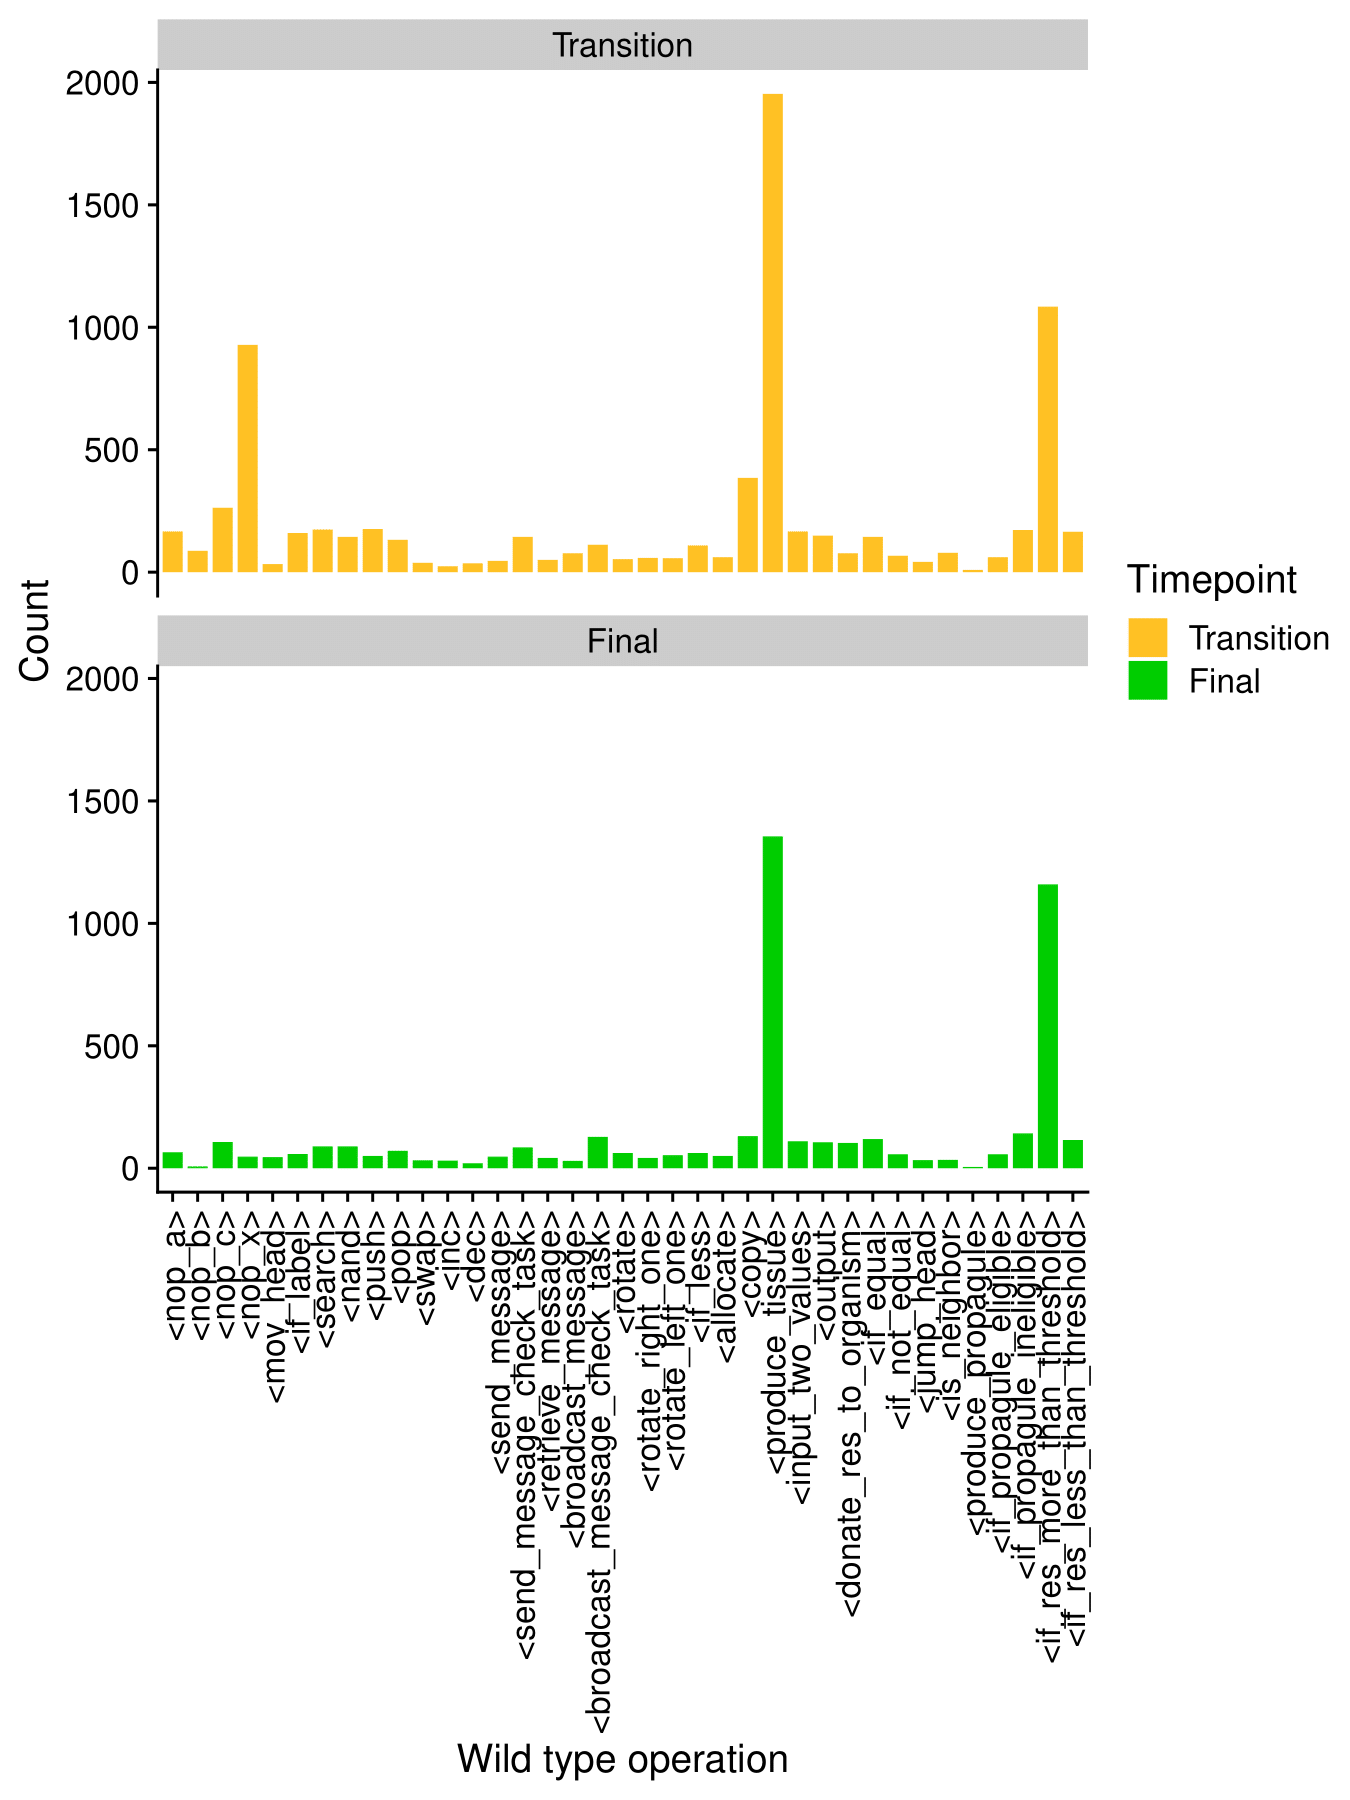
\includegraphics{images/Wildtype_operations_at_transition_and_final_time_point_20DEC22.png}
\caption{\label{fig:wt-operation-identities}\textbf{Changes in replaced wild-type operation identities from the transition to final time point.} The number of times that replacement of different wild-type operations caused reversion to unicellularity.}
\end{figure}

\begin{figure}
\centering
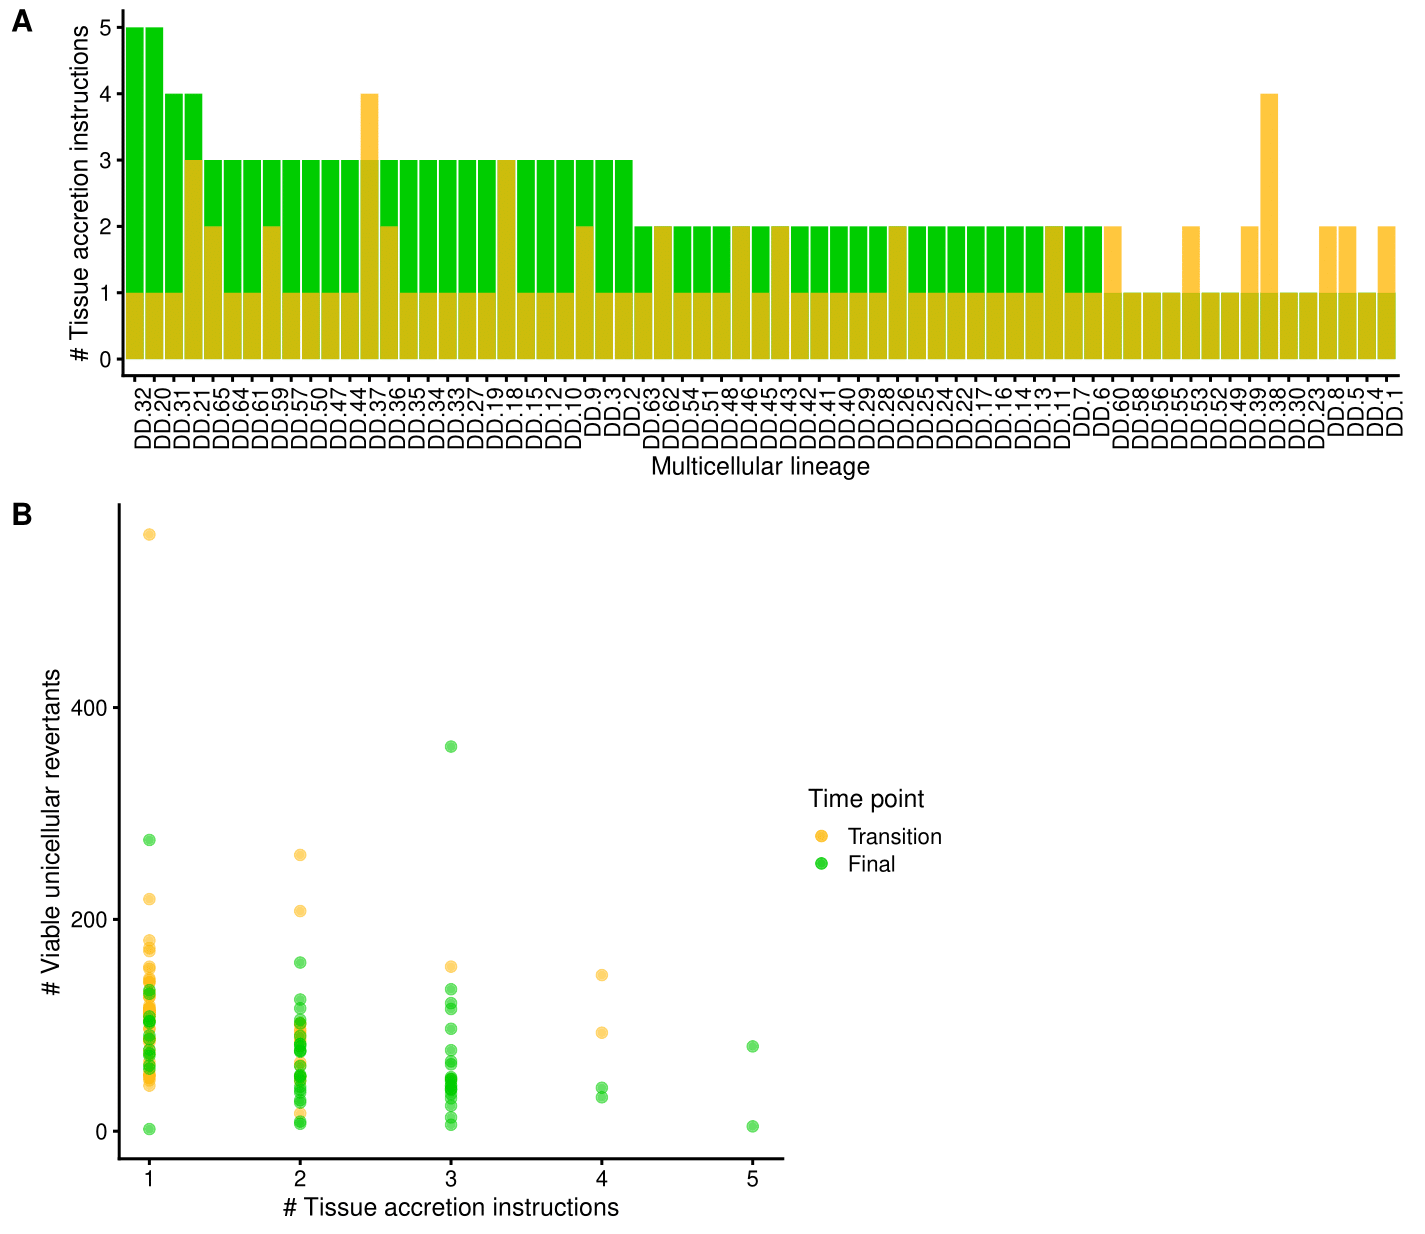
\includegraphics{images/Redundant_tissue_accretion_operations_23DEC22.png}
\caption{\label{fig:redundant-tissue-accretion-instructions}\textbf{Effect of redundant tissue accretion instructions.} To investigate the possibility that redundant tissue accretion instruction operations could reduce the number of viable reversion mutations, we examined the genomes of multicells at the transition (yellow) and final (green) time point. (\textbf{A}) A comparison of the number of tissue accretion instructions found in each genome. (\textbf{B}) The effect of tissue accretion instruction copy number on the number of viable unicellular revertants.}
\end{figure}

\hypertarget{fidelity}{%
\section{Fidelity}\label{fidelity}}

We directly measure the per site mutation rate (\(\mu\)) to assess the fidelity of replication in both multicellular and unicellular genotypes. To do this, we record parent and offspring propagule genomes for each replication event that occurs during our growth assays. Each pair of parent and offspring genomes is then aligned using the aphid R package \citep{aphid} and the instruction equivalent of single nucleotide polymorphisms (SNPs) are called wherever there is a mismatch. To restrict our analyses to mutations that could have been the result of either dirty work or the basal mutation rate we record only these SNPs (insertions and deletions are ignored, for example, as they are the result of errors in the copy loop and not from the effects of dirty work). Finally, duplicate mutation calls are removed by comparing SNPs found in offspring derived from the same parent. We repeat this process 100 times for each genotype. We calculate \(\mu\) as the total number of unique mutations divided by the number of aligned positions from all offspring genomes. Fidelity is reported as one minus the per site mutation rate (i.e., \(1 - \mu\)).

\begin{figure}
\centering
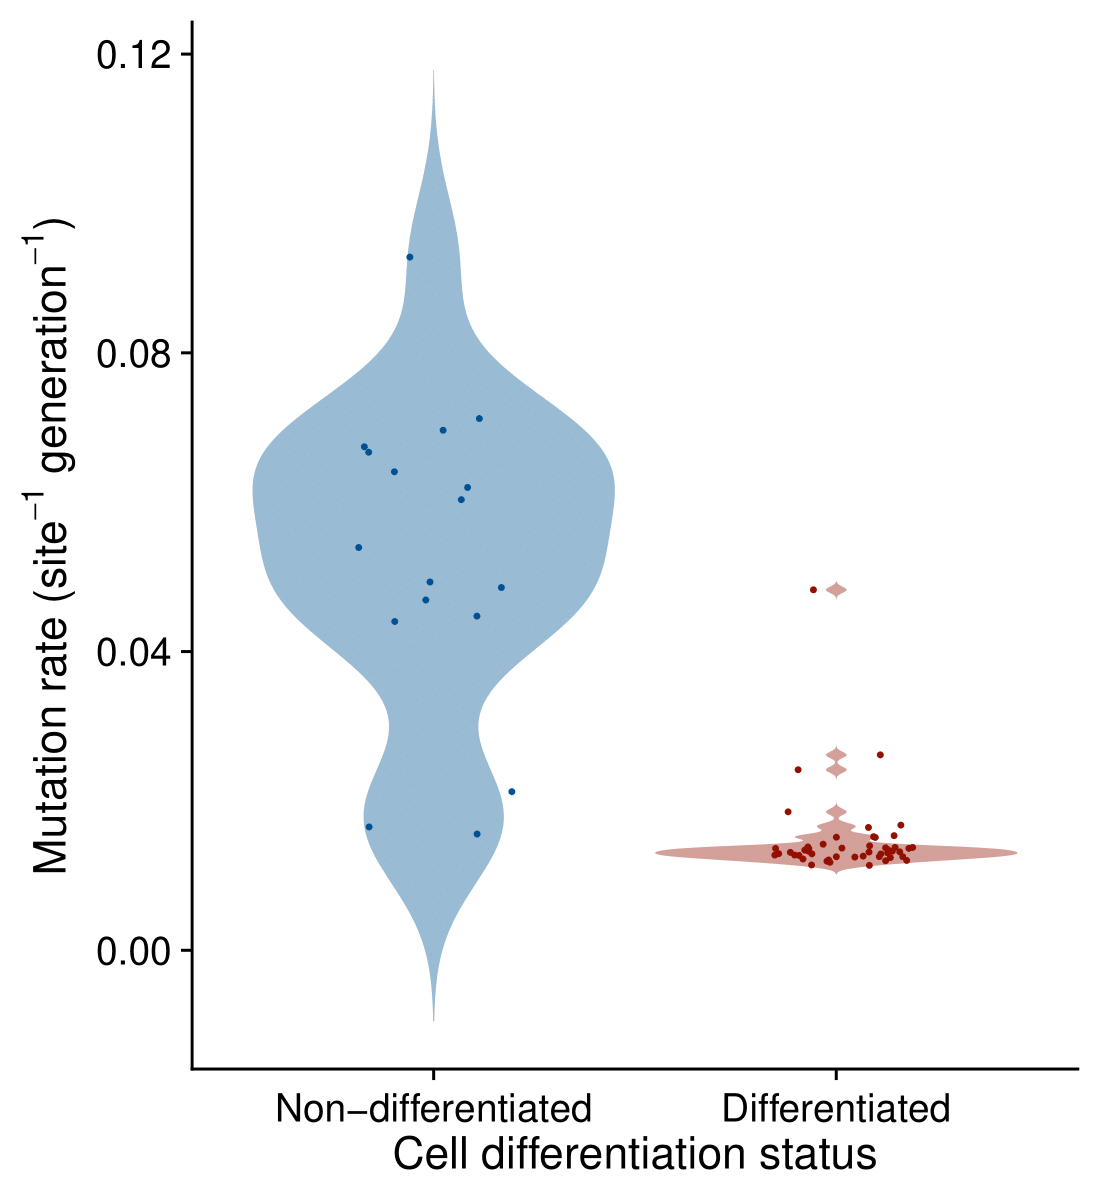
\includegraphics{images/Mutation_rate_by_cell_differentation_status_27JULY20.png}
\caption{\label{fig:mutation-rates}\textbf{Mutation rate by cell differentiation status.}}
\end{figure}

\begin{figure}
\centering
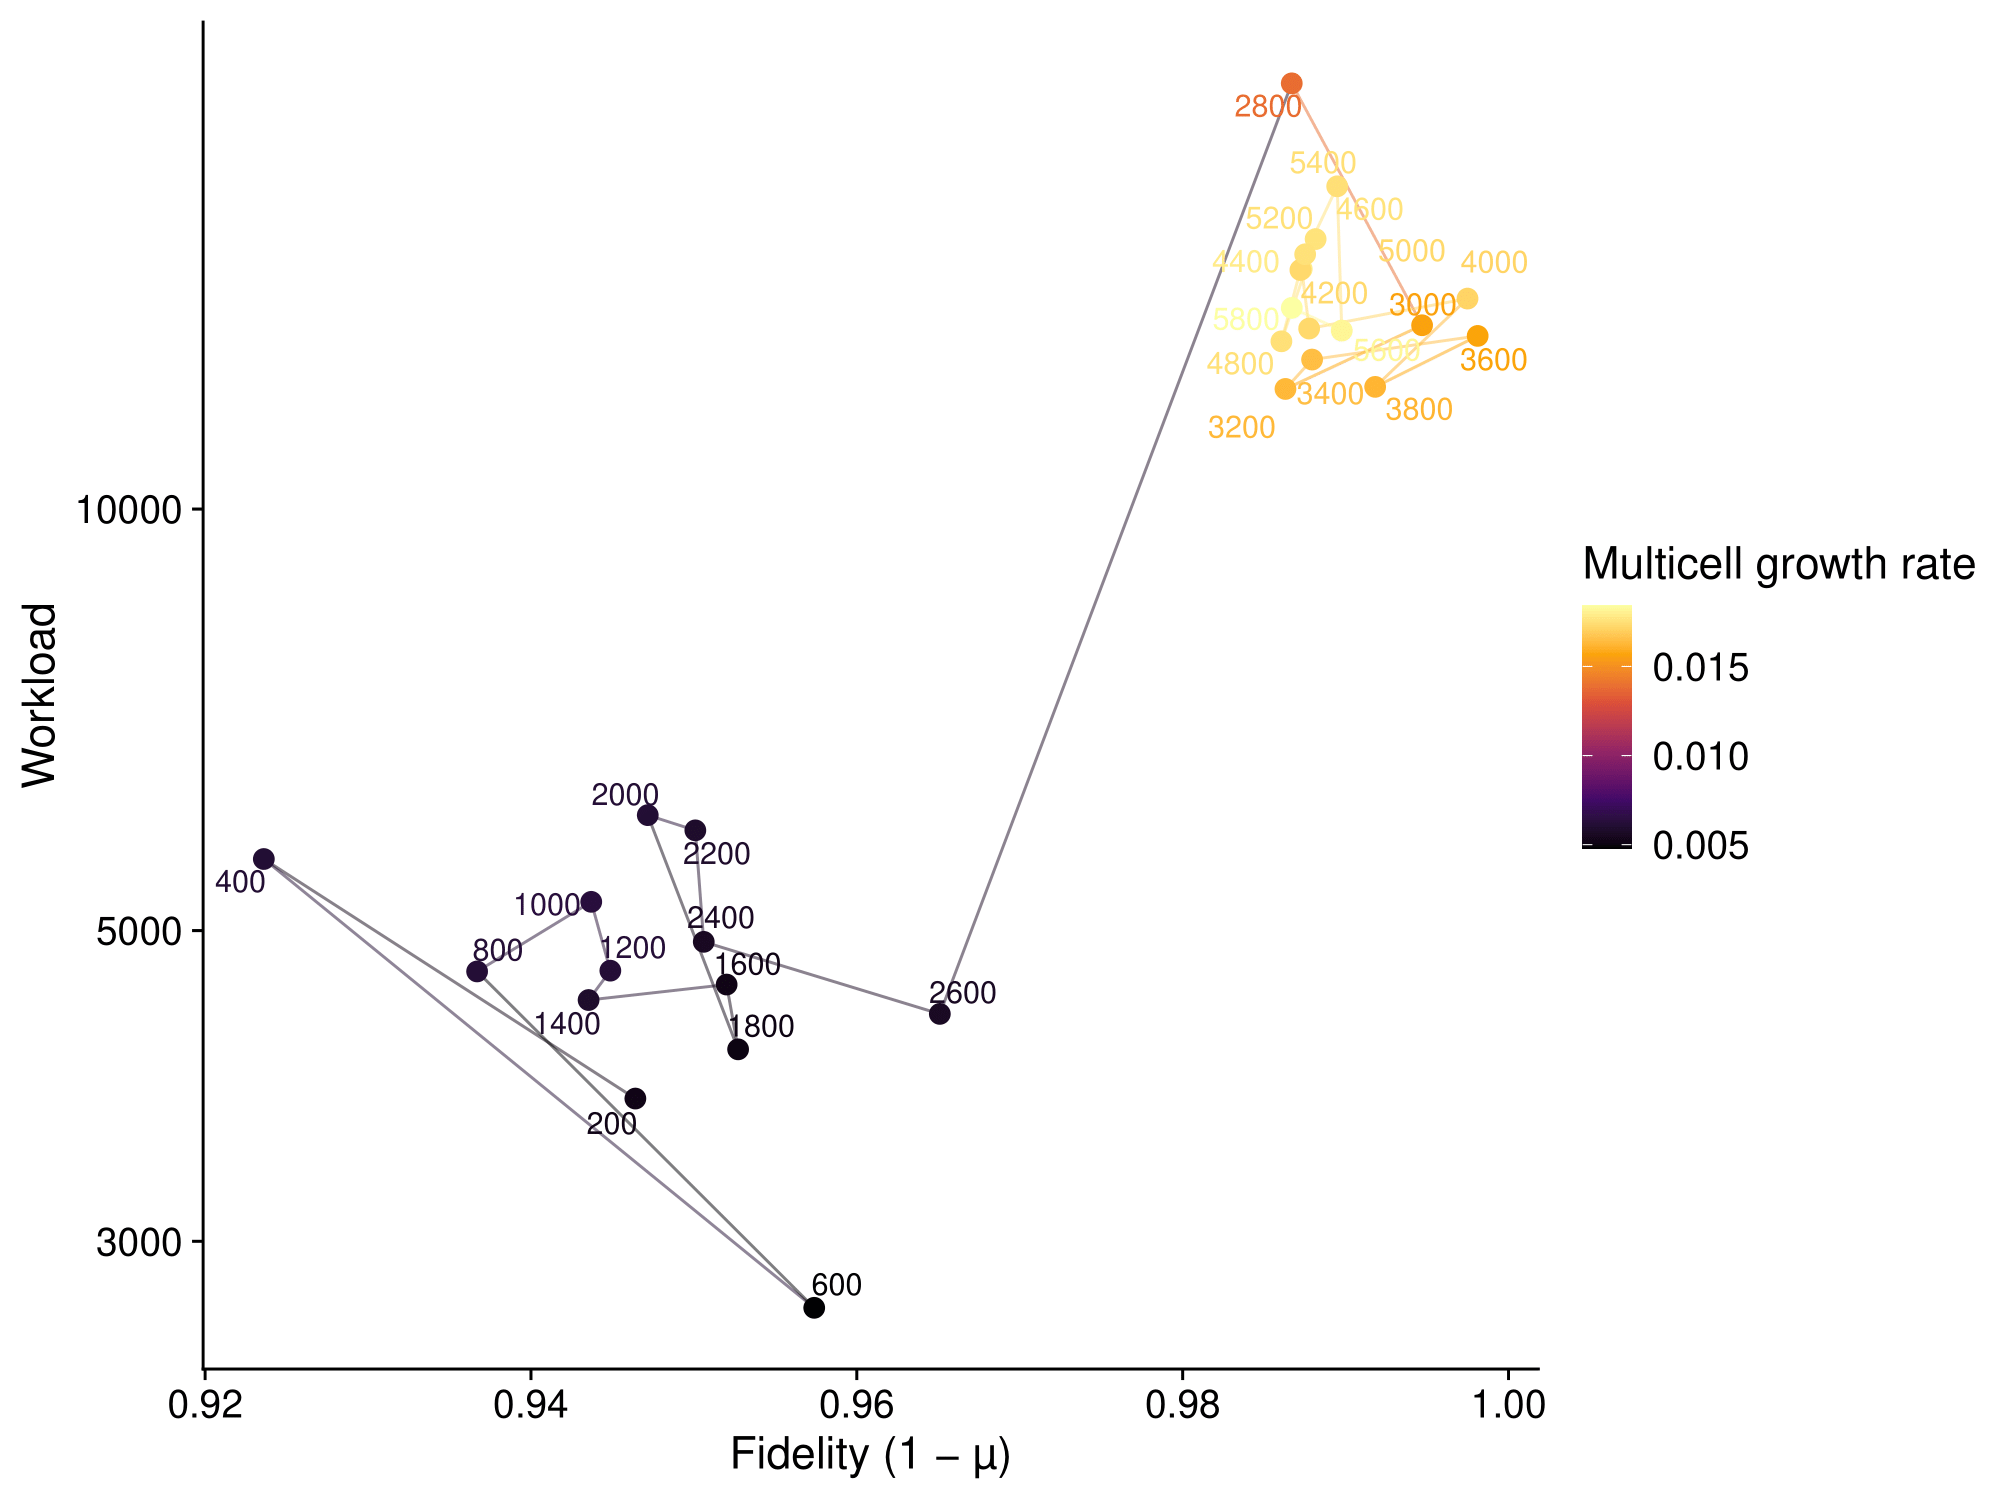
\includegraphics{images/Workload_by_fidelity_case_study_3416_30JULY20.png}
\caption{\label{fig:case-study-over-time-mutation-rates}\textbf{Evolutionary trajectory of a case study population (3416) in workload and fidelity space.}}
\end{figure}

\hypertarget{effect-of-time-spent-evolving-as-a-multicell}{%
\section{Effect of time spent evolving as a multicell}\label{effect-of-time-spent-evolving-as-a-multicell}}

In the main text, we treated all lineages that had evolved multicellularity by the end of their evolutionary run equally. However, we observed considerable variation in the time at which multicellularity evolved and this could lead to differences in entrenchment because genomes would spend different periods of time evolving in a multicellular context \citep{libby2016stabilizing}. To test this prediction, we examined how several key parameters in our study (entrenchment, number of unicellular revertants, revertant relative fitness, revertant growth rate, and multicell growth rate) changed as a function of the number of generations a population spent evolving as a multicell. Consistent with predictions, entrenchment increased significantly with greater time spent evolving as a multicell (Fig. \ref{fig:dw-time-as-mc}A; Spearman's rank-order correlation, \(\rho=0.3\), \(p=0.02\)). Only the change in the number of unicellular revertants did not show a significant correlation with time spent evolving as a multicell (Fig. \ref{fig:dw-time-as-mc}B; Spearman's rank-order correlation, \(\rho=0.08\), \(p=0.53\)). The change in unicell revertant relative fitness declined strongly as a function of time spent evolving as a multicell (Fig. \ref{fig:dw-time-as-mc}C; Spearman's rank-order correlation, \(\rho=-0.34\), \(p=5.5e-3\)) despite the positive correlation between revertant growth rate and time as multicell (Fig. \ref{fig:dw-time-as-mc}D; Spearman's rank-order correlation, \(\rho=0.34\), \(p=6.1e-3\)) because the growth rate improvements were vastly outstripped by those of their multicellular progenitor strains (Fig. \ref{fig:dw-time-as-mc}E; Spearman's rank-order correlation, \(\rho=0.86\), \(p<2.2e-16\)).

\begin{figure}
\centering
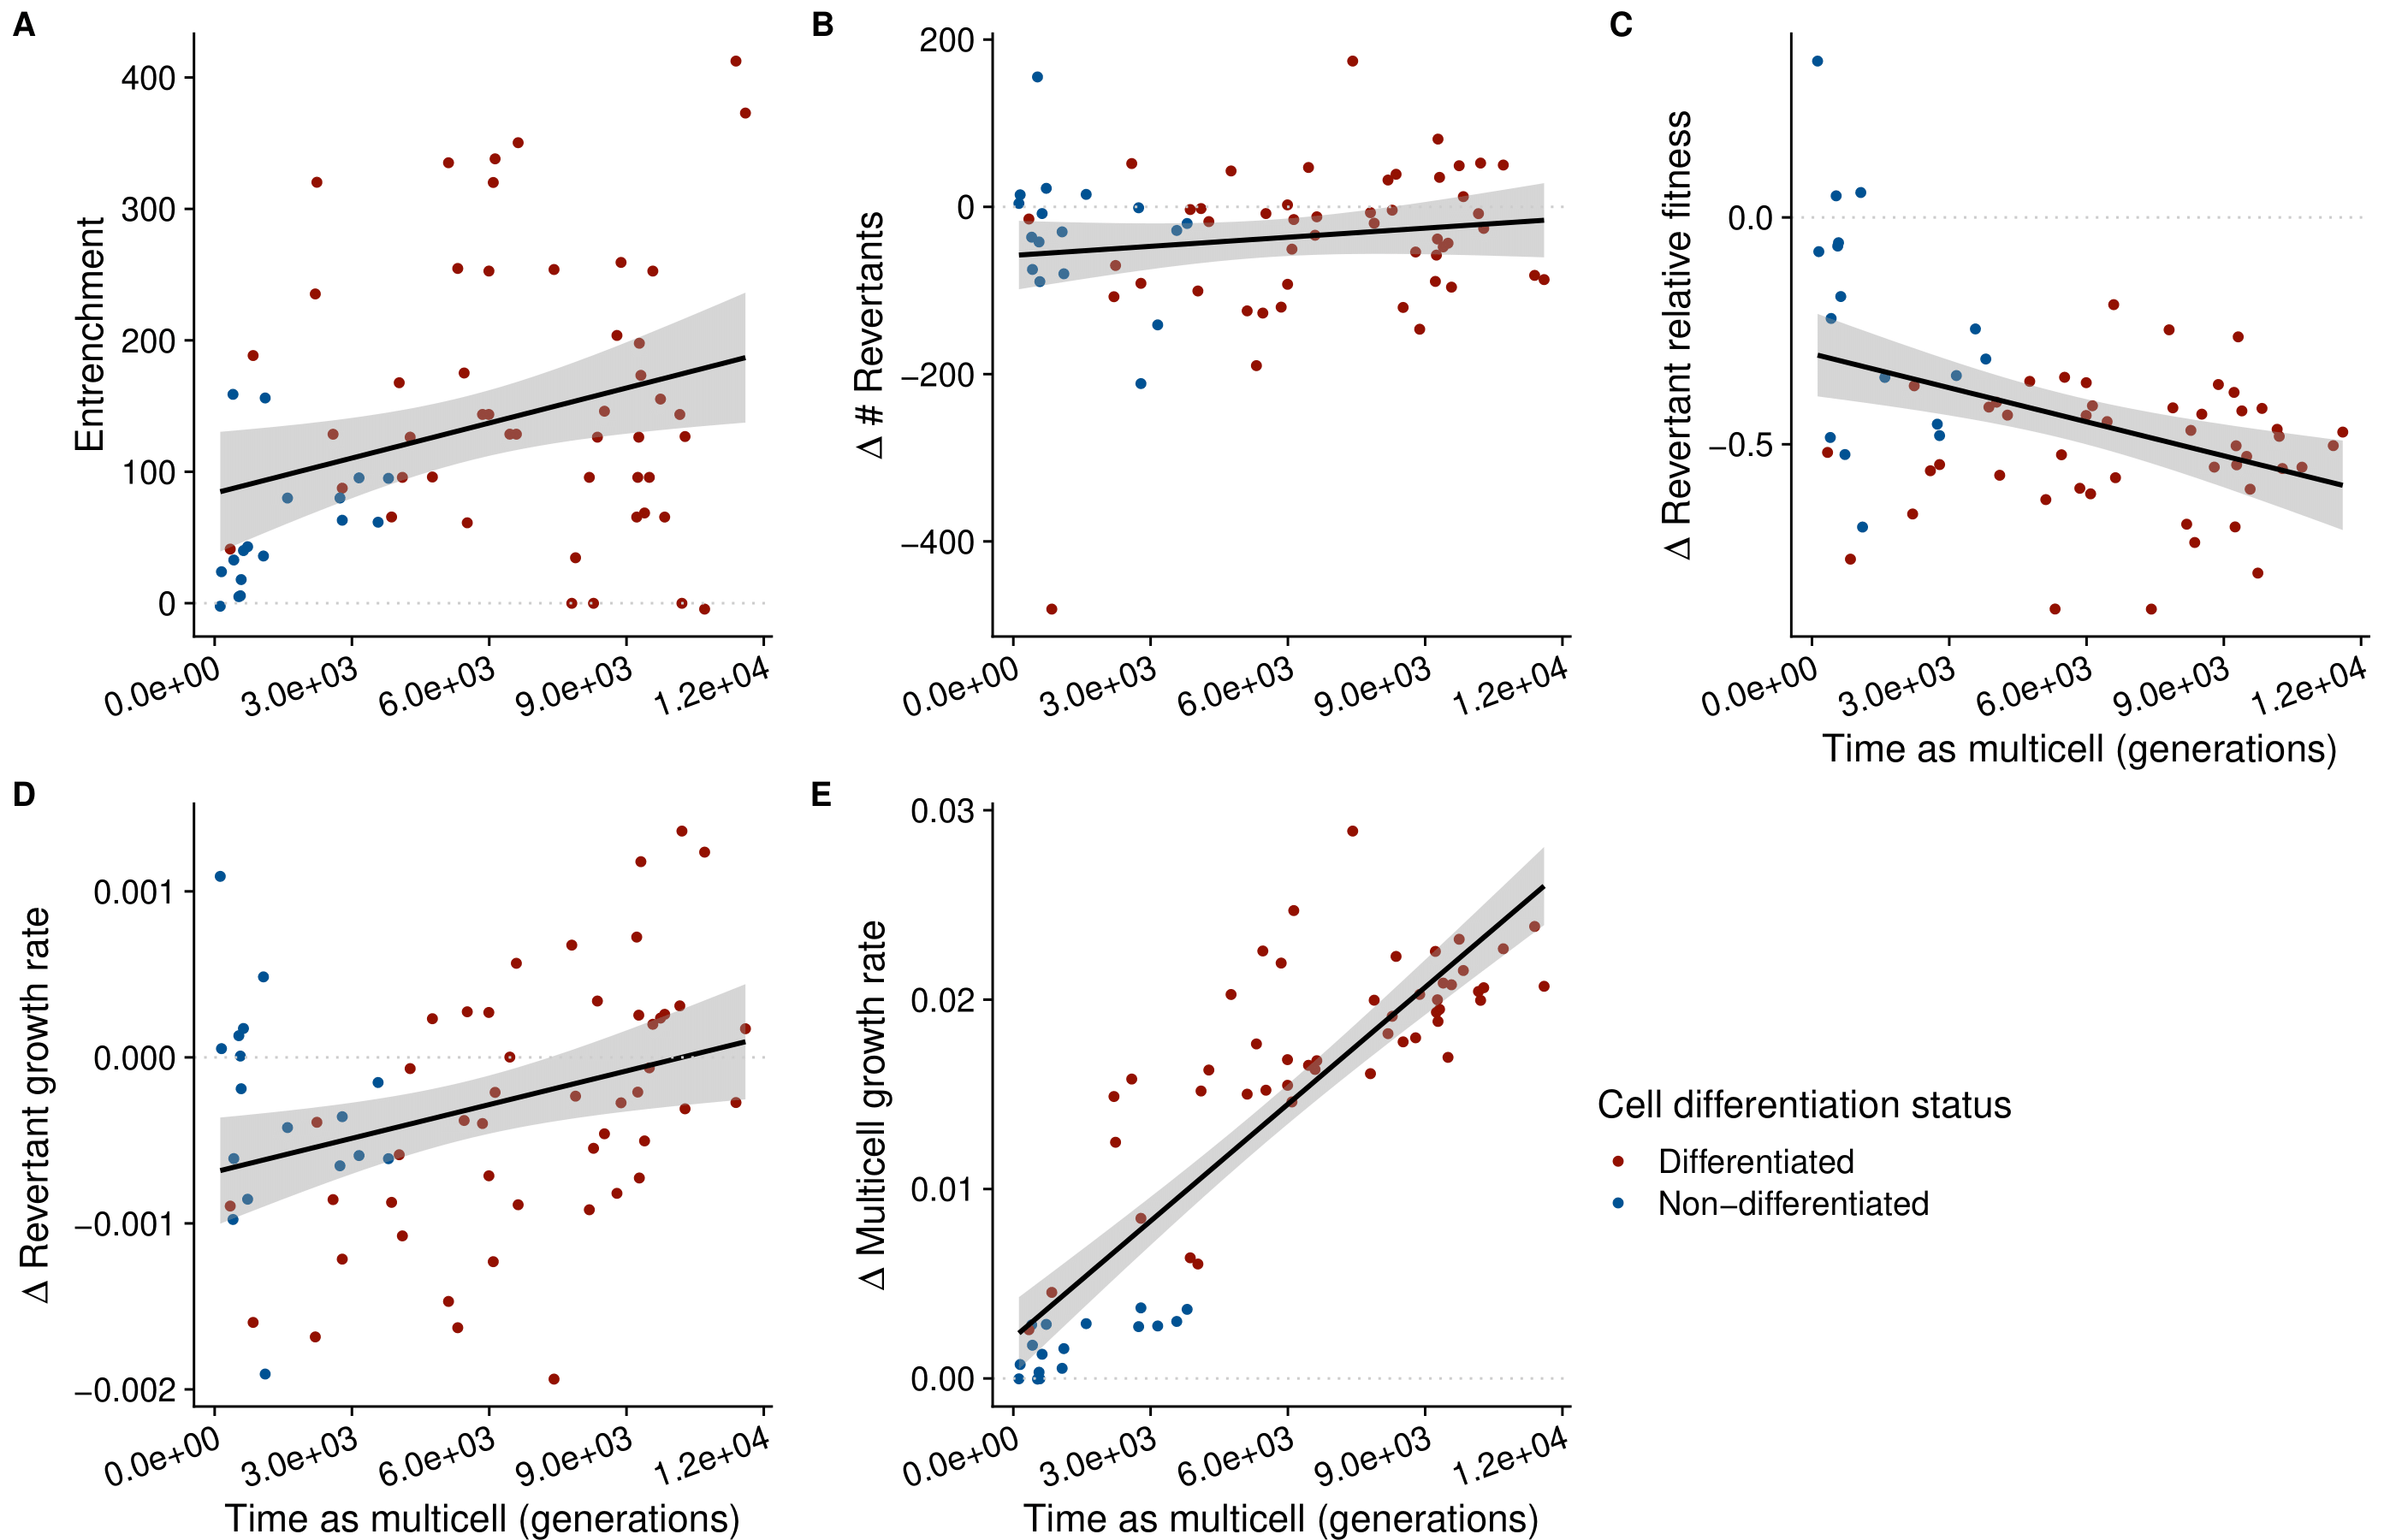
\includegraphics{images/Figure_S8_Time_as_multicell_10NOV22.png}
\caption{\label{fig:dw-time-as-mc}\textbf{Effect of time spent evolving as a multicell.} We examine the correlation between time spent evolving as a multicell and the change in five key parameters in our experiment: entrenchment (\textbf{A}), number of unicellular revertants (\textbf{B}), revertant relative fitness (\textbf{C}), revertant growth rate (\textbf{D}), and multicell growth rate (\textbf{E}). Lineages that evolved germ-soma differentiation appear in red, undifferentiated lineages in blue.}
\end{figure}

\hypertarget{distributed-dirt-model}{%
\chapter{Distributed Dirt Model}\label{distributed-dirt-model}}

The distributed dirt model disrupts the forces underpinning division of labor by separating the performance of a mutagenic task from its mutagenic consequences. In particular, if a cell within an organism performs a mutagenic task, the performing cell accrues the resource from the task, but the cell with the least amount of mutagenic damage is probabilistically mutated and thus is assigned ``the dirt.'\,'

The other parameters within the experiment remain exactly the same as the central division of labor experiment. Cells are still able to communicate, perform tasks, tissue accrete, produce propagules, and become propagule-ineligible. Accordingly, the following downstream analyses were conducted in exactly the same way as described for the Dirty Work experiment: calculating entrenchment (Fig. \ref{fig:dd-entrench-comparison}), filtering revertants (Figs. \ref{fig:dd-filter-1-reevolving-multicellularity}), \ref{fig:dd-filter-2-failure-to-divide}), and plotting the distribution of fitness effects of reversion mutations (Fig. \ref{fig:dd-DFERMs}).

Using the combined datasets from the ``Dirty work'' treatment and the ``Distributed dirt'' treatment, we also examined the overall correlations between key parameters in our system that affect either entrenchment or unicellular revertant fitness (Figs. \ref{fig:Entrenchment-vs-num-revertants-rel-fitness}, \ref{fig:Relative-fitness-vs-uni-and-multi-growth-rates}).

\begin{figure}
\centering
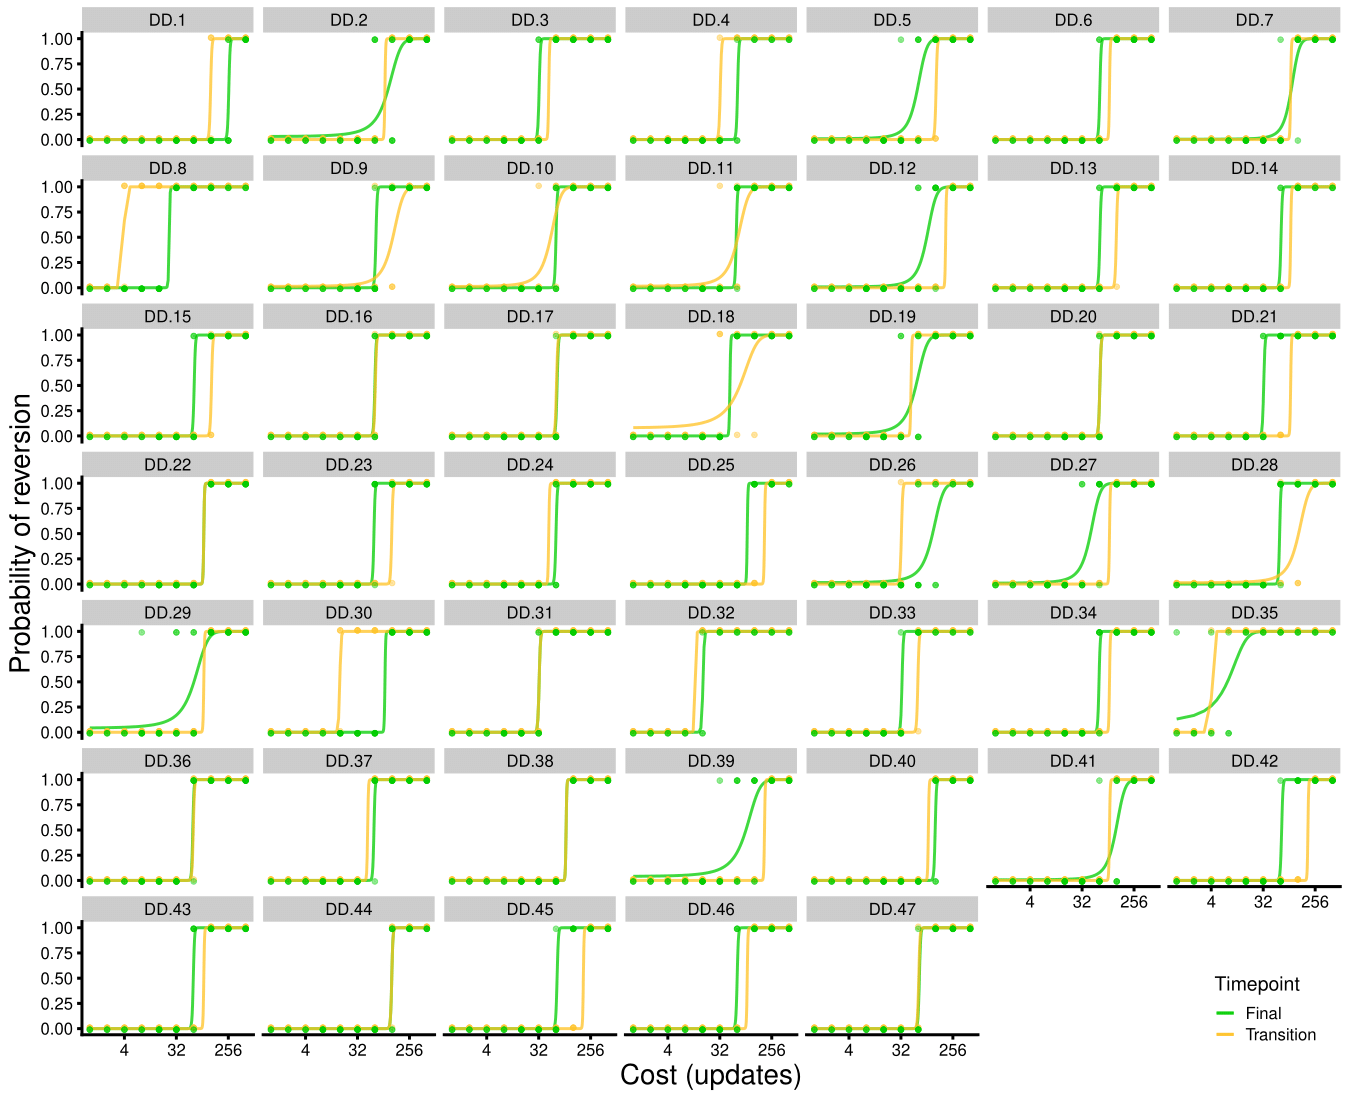
\includegraphics{images/Figure_S10_Dist_Dirt_Entrenchment_20DEC22.png}
\caption{\label{fig:dd-entrench-comparison}\textbf{A comparison of the stability of multicellularity at the transition and final time points of our Distributed Dirt evolution experiment.} The stability of multicellularity was measured for each of the 47 genotypes that evolved multicellularity at the transition (yellow) and final (green) time points of our experiment. The full range of cost values is shown with the outcomes of each replicate plotted as an indicator variable of the dominance of unicellular revertants. Logistic fits of the indicator variable are shown in yellow and green, representing the transition and final time points, respectively.}
\end{figure}

\begin{figure}
\centering
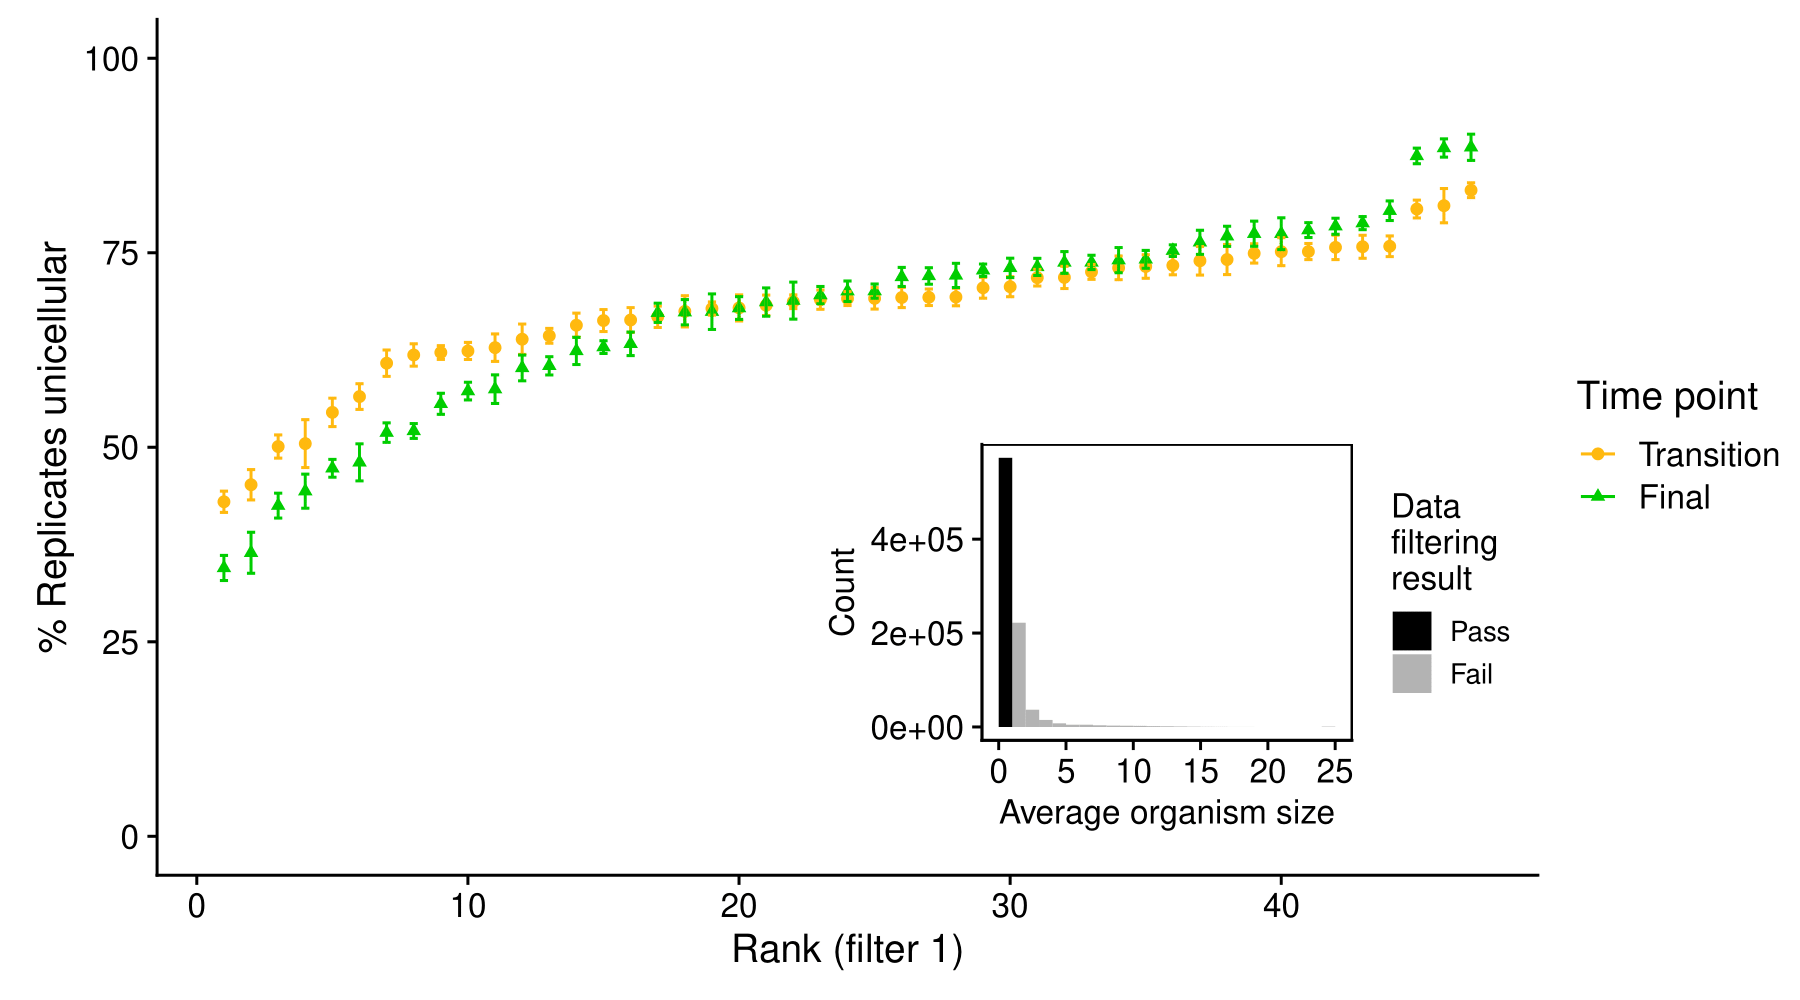
\includegraphics{images/Figure_S11_Dist_dirt_Populations_that_re-evolve_multicellularity_NEW_14MAR23.png}
\caption{\label{fig:dd-filter-1-reevolving-multicellularity}\textbf{Filtering unicellular revertants from the ``Distributed Dirt'' experiment that re-evolve multicellularity.} The mean and standard error for the percent of replicate populations that remain unicellular for the transition (yellow) and final (green) time points of our experiment. Unicellular revertant genotypes are grouped according to their multicellular parental genotypes and ranked from least to most replicates that remain unicellluar for each time point independently. (\textbf{Inset}) Schematic representation of our filtering criterion using data aggregated across all genotypes and both time points. We filter out any population in which the average organism size exceeds 1, indicating that multicellularity has re-evolved. Grey color indicates replicates that fail to pass the filter, black indicates those that do.}
\end{figure}

\begin{figure}
\centering
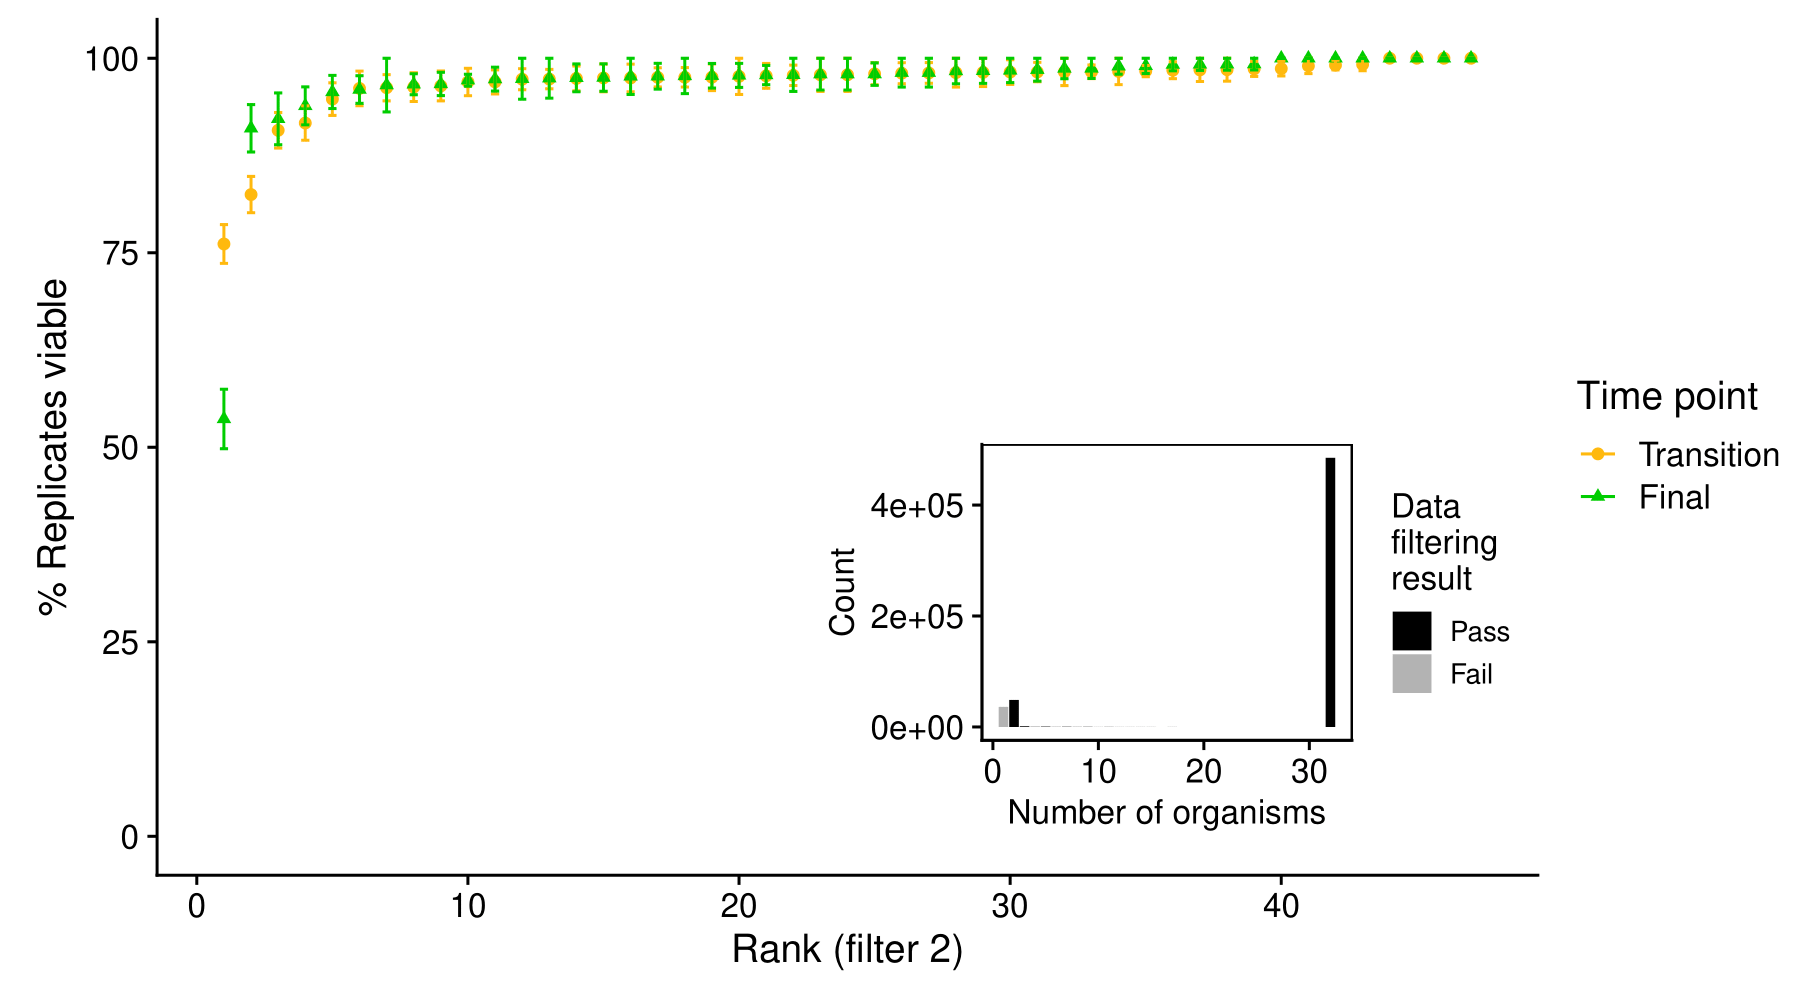
\includegraphics{images/Figure_S12_Dist_dirt_Populations_that_fail_to_divide_NEW_14MAR23.png}
\caption{\label{fig:dd-filter-2-failure-to-divide}\textbf{Filtering unicellular revertants from the ``Distributed Dirt'' experiment that fail to reproduce.} The mean and standard error for the percent of replicate populations that successfully reproduce for the transition (yellow) and final (green) time points of our experiment. Unicellular revertant genotypes are grouped according to their multicellular parental genotypes and ranked from least to most replicates that remain unicellluar for each time point independently. (\textbf{Inset}) Schematic representation of our filtering criterion using data aggregated across all genotypes and both time points. We filter out any population in which the number of organisms at the end of the growth assay is less than 2, indicating that the organism that seeded the population has failed to reproduce. Grey color indicates replicates that fail to pass the filter, black indicates those that do.}
\end{figure}

\begin{figure}
\centering
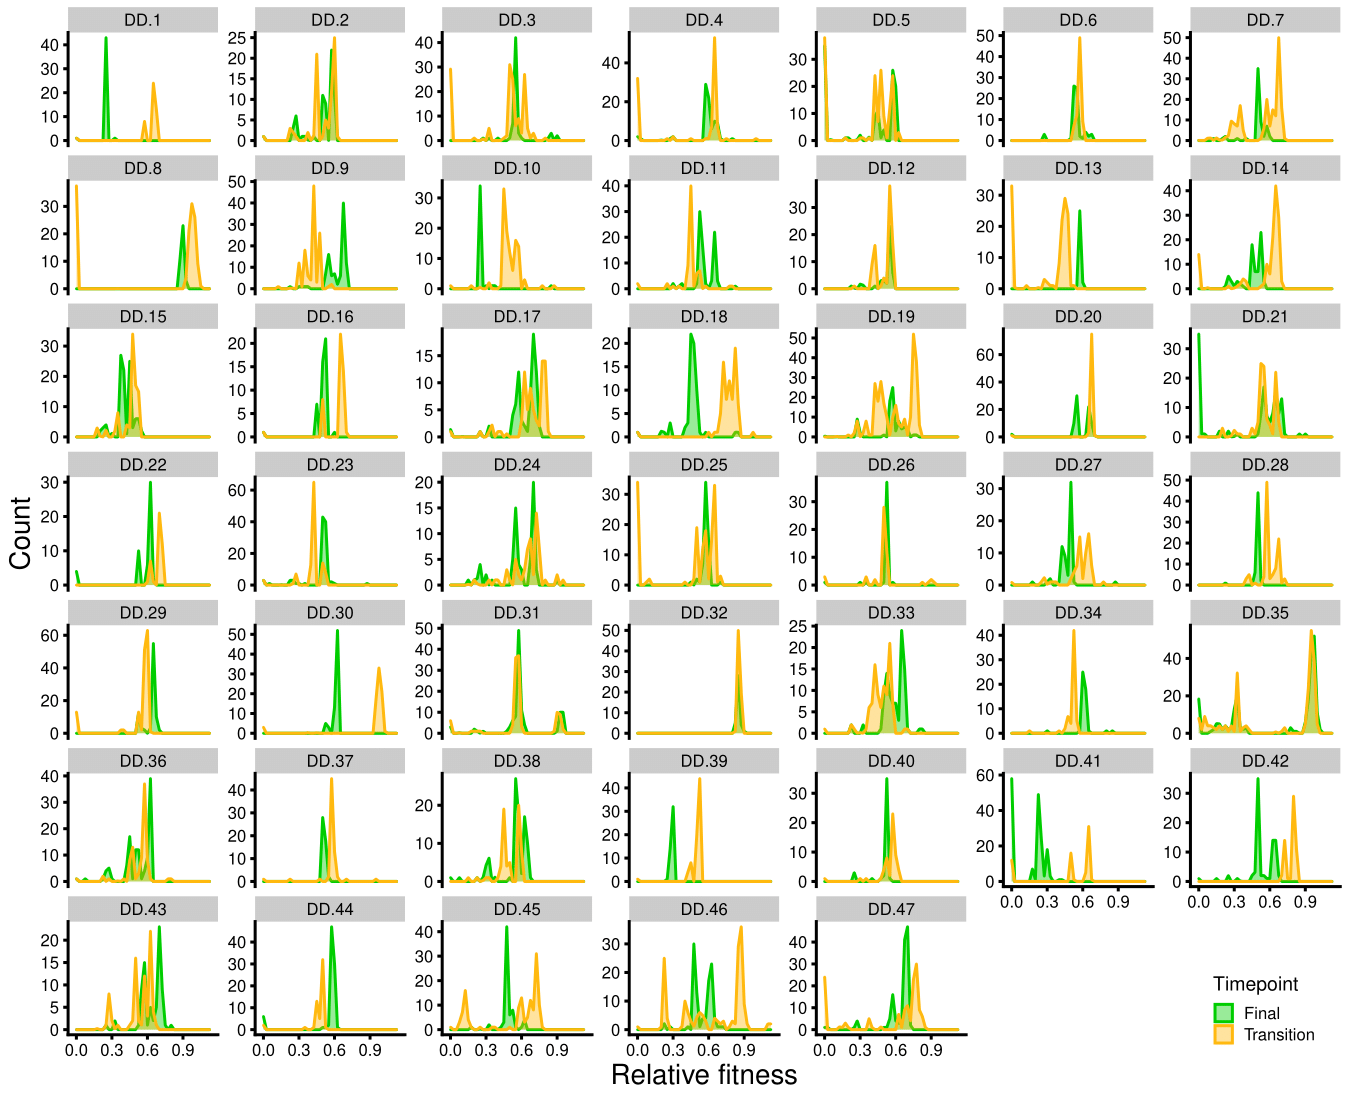
\includegraphics{images/Figure_S13_Dist_Dirt_Relative_fitness_distributions_20DEC22.png}
\caption{\label{fig:dd-DFERMs}\textbf{Distribution of fitness effects of unicellular reversion mutations from the ``Distributed Dirt'' experiment at the transition and final time points.} The empirical distribution of fitness effects of reversion mutations for each lineage that evolved multicellularity in our ``Distributed Dirt'' experiment. Yellow indicates the distribution at the transition point, green at the final time point. Counts are proportional to the adjusted number of unicellular revertants.}
\end{figure}

\begin{figure}
\centering
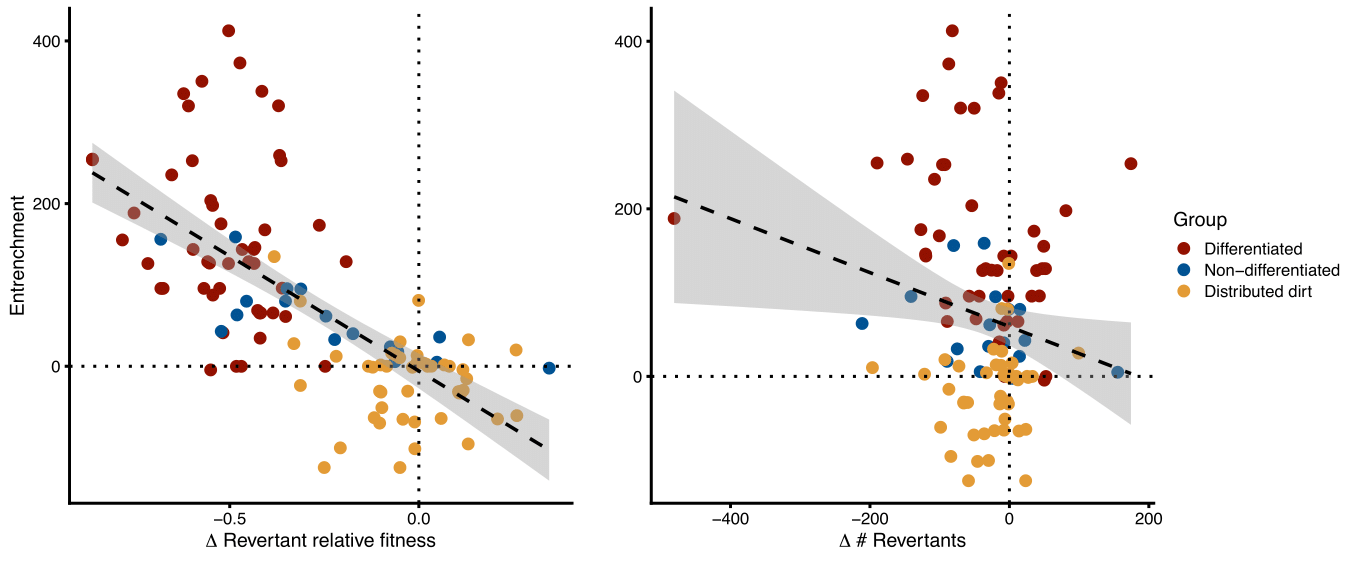
\includegraphics{images/Figure_S8_Entrenchment_vs_num_revertants_and_relative_fitness_12OCT22.png}
\caption{\label{fig:Entrenchment-vs-num-revertants-rel-fitness}\textbf{Entrenchment vs.~relative fitness and number of revertants.} We examine the correlation between entrenchment and its two component parameters: revertant relative fitness (\textbf{A}) and the number of unicellular revertants (\textbf{B}). Differentiated lineages from the dirty-work experiment (red), undifferentiated dirty-work lineages (blue), and the distributed-dirt lineages (gold).}
\end{figure}

\begin{figure}
\centering
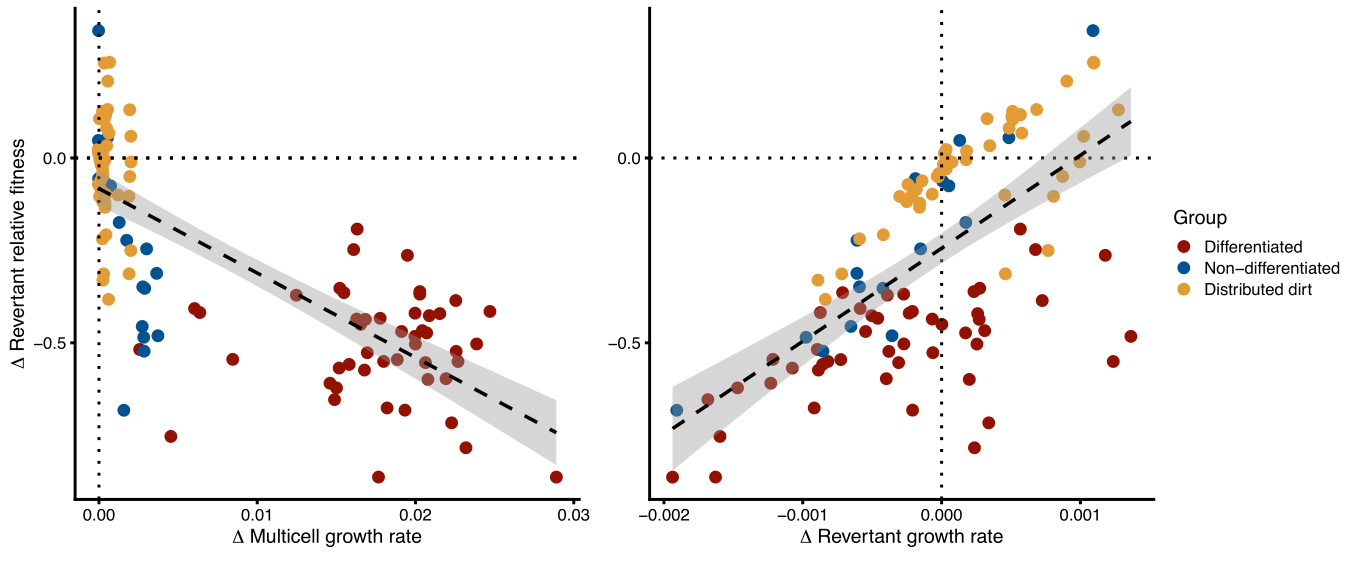
\includegraphics{images/Figure_S9_Relative_fitness_vs_uni_growth_rate_and_multi_growth_rate_12OCT22.png}
\caption{\label{fig:Relative-fitness-vs-uni-and-multi-growth-rates}\textbf{Relative fitness vs.~unicellular growth rate and multicellular growth rate.} We examine the correlation between revertant relative fitness and its two component parameters: the growth rate of the multicellular progenitor strain (\textbf{A}) and the growth rate of the unicellular revertant (\textbf{B}). Differentiated lineages from the dirty-work experiment (red), undifferentiated dirty-work lineages (blue), and the distributed-dirt lineages (gold).}
\end{figure}

  \bibliography{book.bib,packages.bib}

\end{document}
